\documentclass[a4paper,11pt]{report}
\usepackage[utf8]{inputenc}
\usepackage[T1]{fontenc}

%Page margins, header and footer positions
\usepackage{geometry}
 \geometry{
 a4paper,
 total={210mm,297mm},
 left=25mm,
 right=25mm,
 top=30mm,
 bottom=25mm,
 headsep=7mm}

\interfootnotelinepenalty=10000

%To display filling dots in the TOC for all entries
\usepackage[titles]{tocloft}
\renewcommand{\cftsecleader}{\cftdotfill{\cftdotsep}}

%Define new header and footer style
\usepackage{fancyhdr}

\pagestyle{fancy}
\fancyhf{}
\lhead{\color{Gray}{\small{ Best Bike Paths by Luca Suzani, Alberto Spezzapria, Alessio Pesavento}}}
\lfoot{\textcolor{Gray}{\small{Copyright © 2025, Luca Suzani, Alberto Spezzapria, Alessio Pesavento – All rights reserved}}}
\rfoot{\textcolor{Gray}{\thepage}}
\renewcommand{\headrulewidth}{0pt}

%PACKAGES
\usepackage{wasysym}
\usepackage{pifont}

\newcommand{\supported}{\ding{52}\xspace}
\newcommand{\unsupported}{\ding{55}\xspace}
\newcommand{\partsupported}{\textcolor{black!40}{\ding{52}}\xspace}
\newcommand{\lowsupported}{\textcolor{black!20}{\ding{52}}\xspace}
\newcommand{\unknowsupported}{\textbf{?}\xspace}

%Font: Times
\usepackage{times}
%Change monospaced font
\renewcommand{\ttdefault}{lmtt}

%tables
\usepackage{tabu}
\usepackage{tabularx}
\usepackage{ltablex}
\usepackage{longtable}
\usepackage{float} % To allow the use of H modifier in long tables

%landscape mode
\usepackage{pdflscape}
\usepackage{rotating}
\usepackage{caption}

%make landscape mode be sensitive to even and odd pages
%start
\def\myrotate{\ifodd\c@page\else-\fi 90}
\makeatletter
\global\let\orig@begin@landscape=\landscape%
\global\let\orig@end@landscape=\endlandscape%
\gdef\@true{1}
\gdef\@false{0}
\gdef\landscape{%
    \global\let\within@landscape=\@true%
    \orig@begin@landscape%
}%
\gdef\endlandscape{%
    \orig@end@landscape%
    \global\let\within@landscape=\@false%
}%
\@ifpackageloaded{pdflscape}{%
    \gdef\pdf@landscape@rotate{\PLS@Rotate}%
}{
    \gdef\pdf@landscape@rotate#1{}%
}
\let\latex@outputpage\@outputpage
\def\@outputpage{
    \ifx\within@landscape\@true%
        \if@twoside%
            \ifodd\c@page%
                \gdef\LS@rot{\setbox\@outputbox\vbox{%
                    \pdf@landscape@rotate{-90}%
                    \hbox{\rotatebox{90}{\hbox{\rotatebox{180}{\box\@outputbox}}}}}%
                }%
            \else%
                \gdef\LS@rot{\setbox\@outputbox\vbox{%
                    \pdf@landscape@rotate{+90}%
                    \hbox{\rotatebox{90}{\hbox{\rotatebox{0}{\box\@outputbox}}}}}%
                }%
            \fi%
        \else%
            \gdef\LS@rot{\setbox\@outputbox\vbox{%
                \pdf@landscape@rotate{+90}%
                \hbox{\rotatebox{90}{\hbox{\rotatebox{0}{\box\@outputbox}}}}}%
            }%
        \fi%
    \fi%
    \latex@outputpage%
}
\makeatother
%end

%graphics
\usepackage{graphicx}
\usepackage[dvipsnames, table]{xcolor}
%If you upload images from PC, you need to insert code for the path here (different for Windows and Unix OS)

%References
%\usepackage{xpatch}
%\usepackage[backend=biber, style=numeric, citestyle=numeric, sorting=none]{biblatex}
%\addbibresource{main.bib}

%Other
\usepackage{ifthen}
\usepackage{xspace}
\usepackage{enumitem}
\usepackage{amssymb}
% hyperref: hide link colors (prevents red/colored ToC and list entries)
\usepackage[hidelinks]{hyperref}
\newcommand{\comment}[1]{{\color{Red}$\blacktriangleright$ Comment: #1 $\blacktriangleleft$}}


% Some utilities\ldots
\usepackage{soul}
\usepackage{tikz}

\usetikzlibrary{calc}
\usetikzlibrary{decorations.pathmorphing}


\makeatletter

\newcommand{\defhighlighter}[3][]{%
  \tikzset{every highlighter/.style={color=#2, fill opacity=#3, #1}}%
}

\defhighlighter{yellow}{.5}

\newcommand{\highlight@DoHighlight}{
  \fill [ decoration = {random steps, amplitude=1pt, segment length=15pt}
        , outer sep = -15pt, inner sep = 0pt, decorate
       , every highlighter, this highlighter ]
        ($(begin highlight)+(0,8pt)$) rectangle ($(end highlight)+(0,-3pt)$) ;
}

\newcommand{\highlight@BeginHighlight}{
  \coordinate (begin highlight) at (0,0) ;
}

\newcommand{\highlight@EndHighlight}{
  \coordinate (end highlight) at (0,0) ;
}

\newdimen\highlight@previous
\newdimen\highlight@current

\DeclareRobustCommand*\highlight[1][]{%
  \tikzset{this highlighter/.style={#1}}%
  \SOUL@setup
  %
  \def\SOUL@preamble{%
    \begin{tikzpicture}[overlay, remember picture]
      \highlight@BeginHighlight
      \highlight@EndHighlight
    \end{tikzpicture}%
  }%
  %
  \def\SOUL@postamble{%
    \begin{tikzpicture}[overlay, remember picture]
      \highlight@EndHighlight
      \highlight@DoHighlight
    \end{tikzpicture}%
  }%
  %
  \def\SOUL@everyhyphen{%
    \discretionary{%
      \SOUL@setkern\SOUL@hyphkern
      \SOUL@sethyphenchar
      \tikz[overlay, remember picture] \highlight@EndHighlight ;%
    }{%
    }{%
      \SOUL@setkern\SOUL@charkern
    }%
  }%
  %
  \def\SOUL@everyexhyphen##1{%
    \SOUL@setkern\SOUL@hyphkern
    \hbox{##1}%
    \discretionary{%
      \tikz[overlay, remember picture] \highlight@EndHighlight ;%
    }{%
    }{%
      \SOUL@setkern\SOUL@charkern
    }%
  }%
  %
  \def\SOUL@everysyllable{%
    \begin{tikzpicture}[overlay, remember picture]
      \path let \p0 = (begin highlight), \p1 = (0,0) in \pgfextra
        \global\highlight@previous=\y0
        \global\highlight@current =\y1
      \endpgfextra (0,0) ;
      \ifdim\highlight@current < \highlight@previous
        \highlight@DoHighlight
        \highlight@BeginHighlight
      \fi
    \end{tikzpicture}%
    \the\SOUL@syllable
    \tikz[overlay, remember picture] \highlight@EndHighlight ;%
  }%
  \SOUL@
}

\makeatother

% Common abbrev. are set as commands to ensure proper spacing after the dot
\RequirePackage{xspace}
\newcommand{\ie}{i.e.\@\xspace}
\newcommand{\aka}{a.k.a.\@\xspace}
\newcommand{\Ie}{I.e.\@\xspace}
\newcommand{\cf}{cf.\@\xspace}
\newcommand{\Cf}{Cf.\@\xspace}
\newcommand{\eg}{e.g.\@\xspace}
\newcommand{\Eg}{E.g.\@\xspace}
\newcommand{\etal}{et al.\@\xspace}
\newcommand{\etc}{etc.\@\xspace}
\newcommand{\wrt}{w.r.t.\@\xspace}
\newcommand{\Wrt}{W.r.t.\@\xspace}



\date{}

\usepackage{multirow}

\usepackage{listings}
\usepackage{xcolor}

% Definizione colori per il codice
\definecolor{codegreen}{rgb}{0,0.6,0}
\definecolor{codegray}{rgb}{0.5,0.5,0.5}
\definecolor{codepurple}{rgb}{0.58,0,0.82}
\definecolor{backcolour}{rgb}{0.95, 0.95, 0.95}

% Definizione del linguaggio Alloy per evidenziazione sintassi
\lstdefinelanguage{Alloy}{
    keywords={module, sig, enum, fact, pred, assert, run, check, for, but, Int, one, lone, set, seq, extends, in, disj, all, some, no, implies, else, let, sum},
    keywordstyle=\color{blue}\bfseries,
    ndkeywords={True, False, Optimal, Sufficient, Bad, Private, Public},
    ndkeywordstyle=\color{codepurple}\bfseries,
    identifierstyle=\color{black},
    sensitive=true,
    comment=[l]{--},
    morecomment=[l]{//},
    morecomment=[s]{/*}{*/},
    commentstyle=\color{codegreen}\ttfamily,
    stringstyle=\color{red}\ttfamily,
    morestring=[b]",
}

% Stile generale del blocco codice
\lstset{
    backgroundcolor=\color{backcolour},   
    basicstyle=\ttfamily\footnotesize,
    breakatwhitespace=false,         
    breaklines=true,                 
    captionpos=b,                    
    keepspaces=true,                 
    numbers=left,                    
    numbersep=5pt,                  
    showspaces=false,                
    showstringspaces=false,
    showtabs=false,                  
    tabsize=2,
    frame=single
}

\begin{document}

%TITLE PAGE

\begin{titlepage}


%LOGO

{\begin{table}[t!]
\centering
\begin{tabu} to \textwidth { X[1.3,r,p] X[1.7,l,p] }
\textcolor{Blue}
{\textbf{\small{Best Bike Paths, Luca Suzani, Alberto Spezzapria, Alessio Pesavento}}} & 
\includegraphics[scale=0.5]{Images/PolimiLogo}
\end{tabu}
\end{table}}~\\ [7cm]

%TITLE 

\begin{flushleft}

%Replace the text string with your title
{\textcolor{Blue}{\textbf{\Huge{Design Document}}}} \\ [1cm]

\end{flushleft}

\end{titlepage}

%Define deliverable specific info
%Replace cell contents where needed
\begin{table}[h!]
\begin{tabu} to \textwidth { X[0.3,r,p] X[0.7,l,p] }
\hline

\textbf{Deliverable:} & DD\\
\textbf{Title:} & Design Document \\
\textbf{Authors:} & Luca Suzani, Alberto Spezzapria, Alessio Pesavento \\
\textbf{Version:} & 1.0 \\ 
\textbf{Date:} & 22-December-2025 \\
\textbf{Download page:} & https://github.com/Alessio01103/PesaventoSpezzapriaSuzani.git \\
\textbf{Copyright:} & Copyright © 2025, Luca Suzani, Alberto Spezzapria, Alessio Pesavento – All rights reserved \\
\hline
\end{tabu}
\end{table}




\setcounter{page}{2}


%------------------------------------------------------------------------------------------------------------------------------------------------
\newpage
\addcontentsline{toc}{section}{Table of Contents}
\tableofcontents
\newpage
\addcontentsline{toc}{section}{List of Figures}
\listoffigures
\addcontentsline{toc}{section}{List of Tables}
\listoftables

%------------------------------------------------------------------------------------------------------------------------------------------------
\clearpage
\chapter{{Introduction}}
\label{sect:introduction}
\section{Purpose}
The purpose of this document is to provide a comprehensive architectural design for the \textbf{Best Bike Paths (BBP)} system. It serves as the primary bridge between the requirements analysis phase, detailed in the \textit{Requirements Analysis and Specification Document (RASD)}, and the implementation phase.

This document is intended for developers, project managers and testers involved in the project. Its specific goals are to:
\begin{itemize}
    \item Define the \textbf{High-Level Architecture}, identifying the subsystems and their distribution.
    \item Detail the \textbf{Low-Level Components}, specifying their responsibilities, internal logic, and interfaces.
    \item Justify the \textbf{Design Decisions} and architectural styles adopted.
    \item Map the functional requirements to specific software modules to ensure full \textbf{Traceability}.
\end{itemize}

By following this design, it will be possible to implement a scalable, reliable and consistent system that fulfills the user needs regarding cycling safety and path discovery.

\section{Scope}
The \textbf{Best Bike Paths (BBP)} system is a crowdsourcing platform designed to collect, store, search and rank cycling itineraries based on user-generated content and sensor telemetry. The application aims to solve the fragmentation of cycling data by merging individual user tracks into reliable, high-quality public paths.

The scope of the software design covers two main areas:

\begin{enumerate}
    \item \textbf{The Hybrid Client Application:}
    A unified application for Android, iOS, and Web. It is responsible for:
    \begin{itemize}
        \item \textbf{Telemetry Acquisition:}Interfacing with device hardware (GPS, Accelerometer) via a Native Bridge to track routes and detect road irregularities (e.g., potholes) even in background mode.
        \item \textbf{Offline Resilience:} Ensuring data integrity and functionality in areas with poor network coverage through local buffering and synchronization mechanisms.
    \end{itemize}

    \item \textbf{The Serverless Cloud Infrastructure:}
    A managed backend environment responsible for:
    \begin{itemize}
        \item \textbf{Data Consolidation (Merging):} Executing geospatial algorithms to merge conflicting data from multiple users into a "Single Source of Truth" for each path.
        \item \textbf{Dynamic Ranking:} Calculating a suitability score for paths based on safety, road condition, and user feedback freshness.
        \item \textbf{Security:} Enforcing data isolation and access control via Row Level Security (RLS).
    \end{itemize}
\end{enumerate}

The system interacts with external services, specifically third-party \textbf{Weather APIs}, to enrich path metadata. The design excludes the implementation of the physical cycling infrastructure itself, focusing solely on the digital platform to map and evaluate it.

\section{Definitions, Acronyms, and Abbreviations}

\subsection{Definitions}
\begin{itemize}
    \item \textbf{Backend-as-a-Service (BaaS)}: A cloud computing model adopted in this architecture where backend responsibilities (database, authentication, hosting) are outsourced to a managed provider (Supabase), allowing development to focus on frontend logic.
    \item \textbf{Edge Function}: A piece of serverless application logic (e.g., the path merging algorithm) that runs on the cloud provider's infrastructure, triggered by specific database events or HTTP requests.
    \item \textbf{Hybrid Application}: The chosen architectural approach where the mobile app is built using web technologies (React/TypeScript) but executes within a native container to access device hardware.
    \item \textbf{Native Bridge}: The software mechanism (provided by Capacitor) that allows the web-based client code to communicate with the native operating system and access sensors like the Accelerometer and GPS in the background.
    \item \textbf{PostGIS}: An open-source software extender for the PostgreSQL database, used in this project to store, index, and query complex geospatial data (geometries) efficiently.
    \item \textbf{Row Level Security (RLS)}: A security mechanism implemented directly in the database engine that restricts access to specific data rows based on the user's authentication token, eliminating the need for application-level security filters.
    \item \textbf{Thick Client}: An architectural style where the client application (running on the user's device) handles the bulk of data processing, validation, and temporary storage, contrasting with a Thin Client that relies heavily on the server.
\end{itemize}

\subsection{Acronyms}
\begin{itemize}
    \item \textbf{API}: Application Programming Interface.
    \item \textbf{BaaS}: Backend-as-a-Service.
    \item \textbf{CRUD}: Create, Read, Update, Delete.
    \item \textbf{JWT}: JSON Web Token (used for stateless authentication).
    \item \textbf{PWA}: Progressive Web Application.
    \item \textbf{RLS}: Row Level Security.
    \item \textbf{RPC}: Remote Procedure Call (used to invoke Edge Functions).
    \item \textbf{SDK}: Software Development Kit.
    \item \textbf{SPA}: Single Page Application.
    \item \textbf{SQL}: Structured Query Language.
    \item \textbf{WSS}: WebSocket Secure (used for real-time updates).
\end{itemize}

\subsection{Abbreviations}
\begin{itemize}
    \item \textbf{DB}: DataBase.
    \item \textbf{UI}: User Interface.
    \item \textbf{VM}: Virtual Machine.
\end{itemize}


\section{Revision History}
Version 1.0: 07/01/2025

\section{Reference Documents}
\begin{itemize}
    \item \textbf{[1] RDO}: Assignment RDD AY 2025-2026 - Software Engineering 2 Project Assignment, Politecnico di Milano.

    \item \textbf{[2] RASD}: Requirement Analysis and Specification Document for ``Best Bike Paths'', Version 1.0.
        
    \item \textbf{[3] Capacitor Documentation}: Official documentation for the Capacitor native runtime. \\
    Available at: \url{https://capacitorjs.com/docs/}
    
    \item \textbf{[4] TypeScript Language}: Documentation for the TypeScript programming language. \\
    Available at: \url{https://www.typescriptlang.org/}
    
    \item \textbf{[5] Supabase}: Documentation for the open-source Firebase alternative (Backend-as-a-Service). \\
    Available at: \url{https://supabase.com/}
    
    \item \textbf{[6] PostGIS}: Spatial and Geographic objects for PostgreSQL. \\
    Available at: \url{https://postgis.net/}
    
    \item \textbf{[7] Deno}: Documentation for the Deno runtime (used by Supabase Edge Functions). \\
    Available at: \url{https://deno.com/}
    
    \item \textbf{[8] Zod}: TypeScript-first schema declaration and validation library. \\
    Available at: \url{https://zod.dev/}
\end{itemize}
\section{Document Structure}
The following list provides a brief overview of the contents of each chapter in this document:

\begin{itemize}
    \item \textbf{Chapter 1 Introduction:} Provides an overview of the document's purpose and scope, along with definitions of terms and acronyms used throughout the text. It establishes the context for the architectural decisions.
    
    \item \textbf{Chapter 2 Architectural Design:} Constitutes the core of this document. It describes the high-level architecture (Hybrid Client + Serverless Cloud), details the internal software components, their interfaces, and the deployment infrastructure. It also justifies the selected architectural styles and design patterns.
    
    \item \textbf{Chapter 3 User Interface Design:} Presents the visual design of the application through mockups and navigation flow diagrams, illustrating how users interact with the system to perform key tasks.
    
    \item \textbf{Chapter 4 Requirements Traceability:} Provides a mapping between the functional requirements defined in the RASD and the architectural components described in Chapter 2, ensuring that every requirement is addressed by the software design.
    
    \item \textbf{Chapter 5 Implementation, Integration, and Test Plan:} Outlines the strategy for developing the system components, the order of integration, and the testing procedures required to verify the system's correctness and reliability.
    
    \item \textbf{Chapter 6 Effort Spent:} Reports the time spent by each member of the group to contribute to the realization of this document.
\end{itemize}

\section{Use of Generative AI Tools}



%------------------------------------------------------------------------------------------------------------------------------------------------
\clearpage
\chapter{{Architectural Design}}
\label{sect:architectural_design}
\section{Overview}
The \textbf{Best Bike Paths (BBP)} system is architected as a \textbf{Hybrid Mobile Application} supported by a \textbf{Serverless Backend-as-a-Service (BaaS)} infrastructure.

This design strategy allows for a unified codebase (using web technologies like TypeScript/React) to be deployed across both Web and Mobile platforms. Crucially, by leveraging a native runtime bridge (e.g., Capacitor), the application overcomes the limitations of standard web apps. This bridge grants access to native device features, specifically background geolocation and high-frequency motion sensors, which are required for the road Quality Detection and reliability requirements defined in the RASD.

Unlike traditional N-Tier architectures, BBP leverages a thick client model. The client applications contain a significant amount of application logic, communicating directly with the managed cloud database via secure APIs. Complex business logic requiring data aggregation or external integrations is offloaded to edge functions, which execute on-demand in the cloud.

\subsection{High-Level Architecture Description}
The system is composed of two main logical nodes:

\begin{enumerate}
    \item \textbf{Hybrid Client Tier:} This tier includes the unified application running on user devices.
    \begin{itemize}
        \item \textbf{Mobile Deployment (Android/iOS):} The application runs within a native container using Capacitor. It accesses hardware sensors via native plugins to perform precise activity tracking and road irregularity detection even when the device screen is off.
        \item \textbf{Web Deployment:} The same codebase serves as a standard Progressive Web App for path planning and profile management.
        \item \textbf{Responsibilities:}
        \begin{itemize}
            \item Acquisition and pre-processing of raw sensor data (GPS, Accelerometer) via the Native Bridge.
            \item Local data caching (Offline-First) to ensure reliability.
            \item Direct communication with the BaaS provider for CRUD operations.
        \end{itemize}
    \end{itemize}

    \item \textbf{Serverless Cloud Tier:} Hosted on a BaaS platform (e.g., Supabase), acting as the scalable backend. It provides:
    \begin{itemize}
        \item \textbf{Data Persistence:} A PostgreSQL database extended with PostGIS for spatial operations.
        \item \textbf{Authentication:} A built-in identity provider handling OAuth2 and JWT generation.
        \item \textbf{Edge Logic:} Stateless serverless functions that handle background tasks such as path merging, ranking updates, and weather data enrichment.
    \end{itemize}
\end{enumerate}

\subsection{Security Model: Row Level Security (RLS)}
Since clients communicate directly with the database, security is enforced at the database layer using Row Level Security (RLS) policies.
Upon login, the Auth Service issues a JSON Web Token (JWT) to the client, which is included in every database query. The database engine evaluates RLS policies for each row to determine if the operation is permitted. This ensures that "direct access" does not imply "unrestricted access", maintaining strict data isolation and integrity.

\subsection{Platform-Specific Feature Availability}
While the Client Application is developed as a Progressive Web App (PWA) with a shared codebase, the feature set varies depending on the deployment target (Mobile vs Web) due to hardware access constraints:
\begin{itemize}
    \item \textbf{Mobile Application (Android/IOS):} This version utilizes the Capacitor Native Bridge to access low-level hardware APIs. It supports the full feature set, including the Activity Recording module, which requires continuous access to the GPS and Accelerometer sensors even when the application is running in the background or the device screen is off.
    \item \textbf{Web Application (browser):} Accessible via standard web browsers, this version focuses on planning and analysis. Due to browser sandboxing policies and the inability to reliably maintain background processes for sensor sampling, the Activity Recording functionality is disabled. Users can utilize this platform for Path Search, Data Visualization and Profile Management.
\end{itemize}
\section{Component view}
This section details the software components within the Client and Cloud tiers, defining their specific responsibilities and interactions.

\subsection{Hybrid Client Components}
\begin{itemize}
    \item \textbf{Native Bridge (Capacitor):} The architectural boundary between the web code and the native OS. It exposes a unified API to access hardware features. It ensures that the \textbf{Geolocation} and \textbf{Accelerometer} continue to operate reliably even when the application is in the background, bridging the gap between the web runtime and the device hardware.
    
    \item \textbf{Sensor Controller \& Filter:} Responsible for logic related to data acquisition.
    \begin{itemize}
        \item It interfaces with the \textbf{Native Bridge} to subscribe to GPS and Accelerometer streams.
        \item It implements a \textbf{Kalman Filter} to smooth raw GPS coordinates.
        \item It analyzes accelerometer data to detect vertical shocks (road surface irregularities like potholes) and buffers this data locally during activity recording.
    \end{itemize}
    
    \item \textbf{Local Persistence Manager:} Implements the "Offline-First" capability. It uses an embedded database (e.g., SQLite via Capacitor plugin) to store activity traces and pending reports when the network is unavailable. It includes a \textbf{Sync Engine} that monitors network reachability and uploads buffered data to the cloud once connectivity is restored.
    
    \item \textbf{BaaS Client SDK:} The abstraction layer provided by the BaaS platform. It manages the persistent WebSocket connection for real-time updates, handles secure API calls to the database, and automatically refreshes authentication tokens.
    
    \item \textbf{Map \& UI Controller:} Manages the visualization of map tiles and path geometries. It handles user inputs (forms, search queries) and renders the visual feedback for the navigation system.
\end{itemize}

\subsection{Managed Cloud Components (BaaS)}
\begin{itemize}
    \item \textbf{Auth Service (Identity Provider):} Manages user lifecycles (sign-up, login, password recovery). It integrates with third-party OAuth providers (e.g., Google, Facebook) and issues secure JWTs containing user roles and IDs.
    
    \item \textbf{Spatial Database (PostgreSQL + PostGIS):} The central data repository. It is an active component that:
    \begin{itemize}
        \item Enforces \textbf{RLS Policies} to secure data access.
        \item Executes complex \textbf{Spatial Queries} (e.g., \texttt{ST\_DWithin}, \texttt{ST\_Intersects}) natively, allowing clients to efficiently retrieve paths within a specific viewport.
        \item Triggers database events (Webhooks) to activate Edge Functions upon data changes.
    \end{itemize}
    
    \item \textbf{Object Storage:} A specialized file storage system for large binary assets, such as user profile pictures or images attached to path reports.
\end{itemize}

\subsection{Edge Functions}
These are stateless functions triggered by database events or scheduled cron jobs:
\begin{itemize}
    \item \texttt{func\_path\_merging}
    \begin{itemize}
        \item \textbf{Trigger:} Database event (INSERT on \texttt{Activities} or \texttt{Feedbacks} table).
        \item \textbf{Responsibility:} It implements the \textbf{Data Consolidation \& Consensus Logic}. When new data (an activity trace or a manual report) is associated with a path, this function aggregates it with existing reports to determine the path's \texttt{CurrentCondition}. It applies a \textbf{Majority Voting Algorithm} weighted by data freshness (e.g., resolving a conflict where 3 recent reports say "Good" and 1 says "Bad" by marking the segment as "Good") to ensure the status reflects the actual road situation.
    \end{itemize}

    \item \texttt{func\_path\_search}
    \begin{itemize}
        \item \textbf{Trigger:} Direct Client Request.
        \item \textbf{Responsibility:} It implements the \textbf{Search \& Ranking Algorithm} defined in the RASD. When a user queries for a route (specifying Origin and Destination), this function:
        \begin{itemize}
            \item Performs a spatial query to find candidate paths connecting the points.
            \item Dynamically calculates a \textbf{Suitability Score} for each candidate. This score combines the \textbf{Geospatial match} (how well it fits the requested Start/End points) with the \textbf{Path Quality} (derived from the consolidated feedback and applying a time-decay factor to older data).
            \item Returns the list of paths ordered by this score.
        \end{itemize}
    \end{itemize}

    \item \texttt{func\_maintenance\_job}
    \begin{itemize}
        \item \textbf{Trigger:} Scheduled Cron Job (e.g., Nightly).
        \item \textbf{Responsibility:} Periodically applies the \textbf{Time-Decay Function} to the database. It archives or lowers the weight of very old reports/feedbacks to ensure that the \texttt{func\_path\_search} always prioritizes fresh information without needing to process the entire history during every query.
    \end{itemize}

    \item \texttt{func\_weather\_enricher}
    \begin{itemize}
        \item \textbf{Trigger:} Database event (INSERT on \texttt{Activities}).
        \item \textbf{Responsibility:} It securely calls external Meteorological APIs (using backend-only API keys) to fetch weather conditions for the specific time and location of the activity, enriching the path metadata.
    \end{itemize}

    \item \texttt{func\_path\_deduplication}
    \begin{itemize}
        \item \textbf{Trigger:} Direct Client Request (RPC via check\_path\_duplicate)
        \item \textbf{Responsibility:} It implements the \textbf{Geometric Integrity Control Logic.} 
        Before a new manual path is saved to the database, this function receives the geometry drawn by the user and executes a high-performance spatial query to verify the existence of already present public paths that are geometrically identical or extremely similar. It returns the validation result to the client, preventing the creation of redundant duplicates and ensuring path uniqueness within the system.
    \end{itemize}
\end{itemize}

% INSERT DIAGRAM 2.2 HERE
% \begin{figure}[H]
% \centering
% \includegraphics[width=\textwidth]{images/diagram_2_2_components.png}
% \caption{Component View}
% \label{fig:component_view}
% \end{figure}
\section{Deployment view}
The deployment architecture of \textbf{Best Bike Paths} follows a distributed, client-server model relying on a \textbf{Serverless Infrastructure}. This approach minimizes operational overhead, as the backend resources (Database, Auth, Compute) are provisioned and scaled automatically by the Cloud Provider.

The system is deployed across three primary types of nodes:

\begin{enumerate}
    \item \textbf{Mobile User Device (Android/iOS):}
    \begin{itemize}
        \item \textbf{Hardware:} Personal Smartphone.
        \item \textbf{Execution Environment:} Native OS hosting the \textbf{Capacitor Runtime} (WebView).
        \item \textbf{Artifacts:} The \textit{Hybrid Mobile Application} package (\texttt{.apk} / \texttt{.ipa}). This artifact contains the compiled Javascript/React bundle and the native plugins required to access hardware sensors (GPS, Accelerometer). It includes an embedded SQLite database for local persistence.
    \end{itemize}

    \item \textbf{Web User Station (Desktop/Laptop):}
    \begin{itemize}
        \item \textbf{Hardware:} Personal Computer.
        \item \textbf{Execution Environment:} Modern Web Browser (Chrome, Firefox, Safari).
        \item \textbf{Artifacts:} The \textit{Progressive Web Application (PWA)} assets (HTML, CSS, JS bundles) cached by the Service Worker.
    \end{itemize}

    \item \textbf{Managed Cloud Platform (BaaS Provider):}
    \begin{itemize}
        \item \textbf{Hardware:} Distributed Virtualized Clusters (managed by Supabase/AWS).
        \item \textbf{Execution Environment:} Containerized Database Engine and V8 Isolate runtime for Edge Functions.
        \item \textbf{Artifacts:}
        \begin{itemize}
            \item \textit{PostgreSQL Instance:} Stores data and RLS policies.
            \item \textit{Auth Service Instance:} Handles identity management.
            \item \textit{Edge Functions:} Deployed serverless scripts (\texttt{path\_merging}, \texttt{score\_calc}) executed on demand.
        \end{itemize}
    \end{itemize}
\end{enumerate}

\subsection{Network Communication}
Communication between the Client Nodes and the Cloud Platform occurs exclusively over secure standard protocols:

\begin{itemize}
    \item \textbf{HTTPS (TLS 1.3):} For all REST API calls (Database CRUD, RPC functions).
    \item \textbf{WSS (Secure WebSockets):} For real-time event subscriptions (e.g., live feedback updates).
\end{itemize}

\section{Runtime view}
% --- UC1: User Registration ---
\subsubsection*{[UC1] User Registration Sequence Diagram}
\begin{figure}[H]
    \centering
    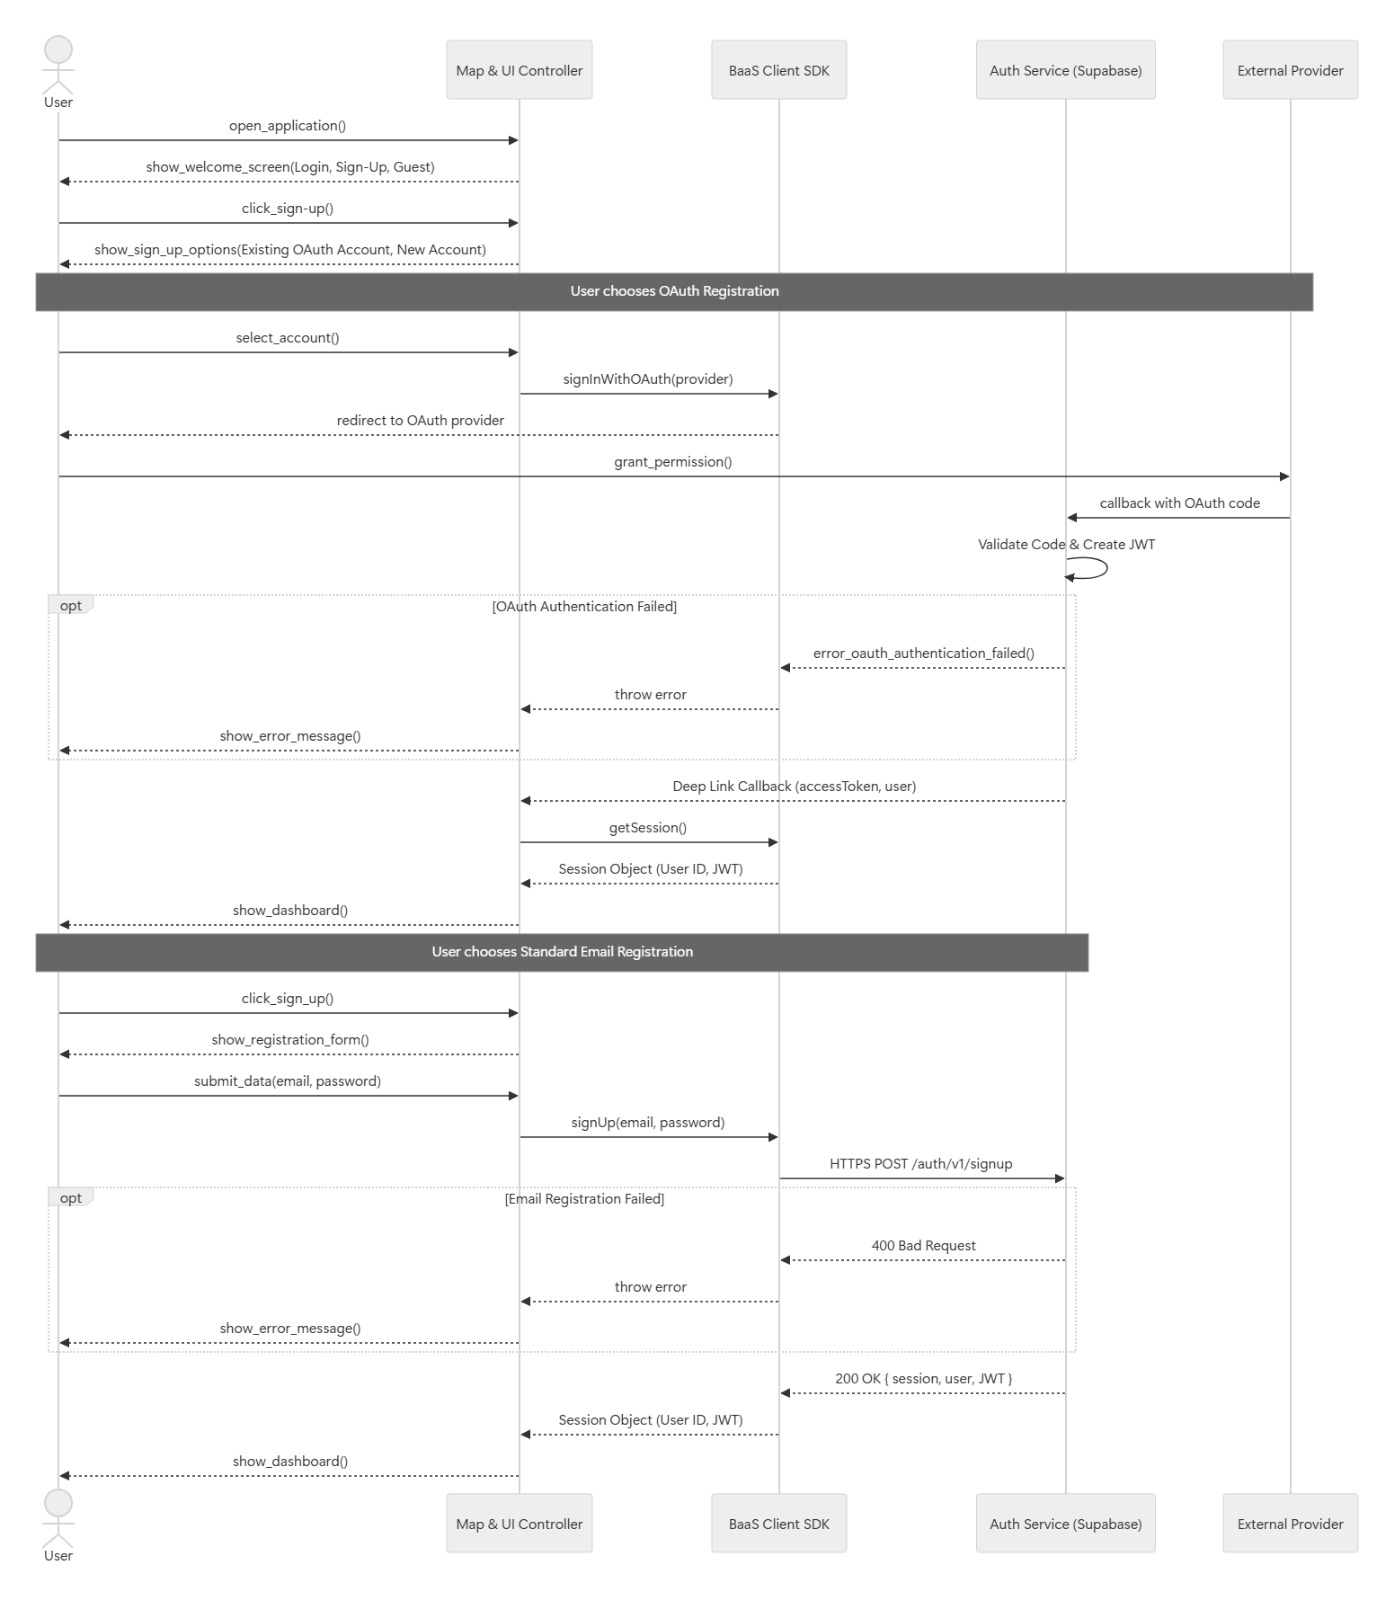
\includegraphics[width=\textwidth]{Images/uc1_sd.jpeg}
    \caption{[UC1] User Registration Sequence Diagram}
    \label{fig:sd_uc1}
\end{figure}
The diagram illustrates the registration process managed by the Auth Service. In the OAuth scenario, the flow delegates authentication to the external provider via redirect and callback (Deep Link). In the Email scenario, the SDK communicates directly with the Supabase API. In both cases, the final result is the acquisition of a valid JWT (JSON Web Token), which is essential for ensuring secure access to the database via RLS policies in subsequent interactions.

% --- UC2: System Access ---
\subsubsection*{[UC2] System Access Sequence Diagram}
\begin{figure}[H]
    \centering
    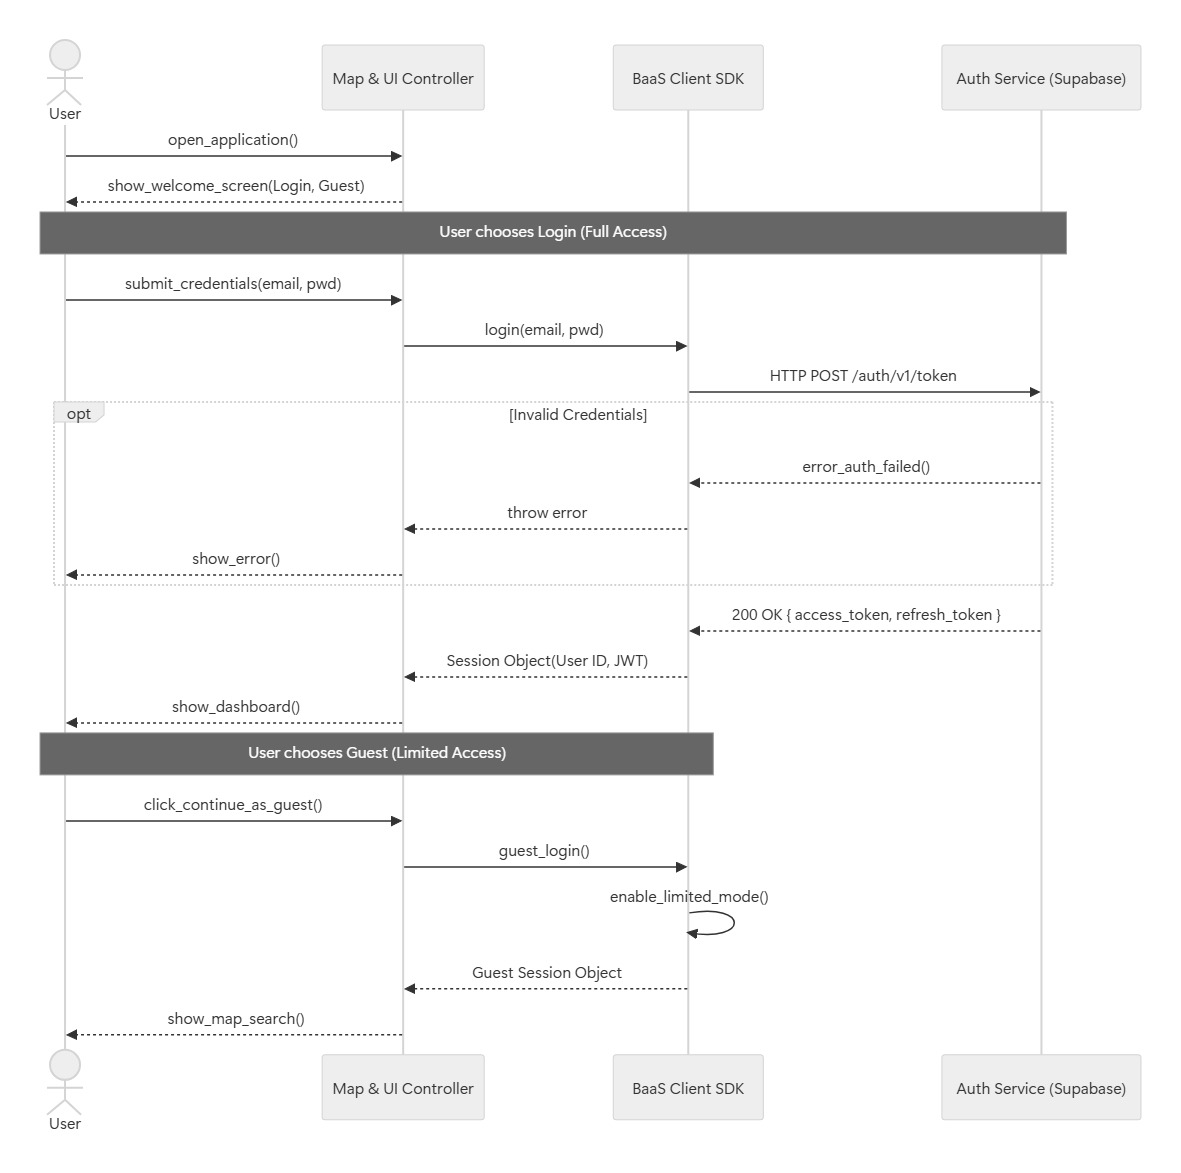
\includegraphics[width=\textwidth]{Images/uc2_sd.jpeg}
    \caption{[UC2] System Access Sequence Diagram}
    \label{fig:sd_uc2}
\end{figure}
This diagram depicts the session negotiation process. For registered users, the BaaS Client SDK exchanges credentials for a persistent session token. For Guest users, the SDK initializes a local session in "Limited Mode," which disables write calls to the database and restricts access exclusively to public search APIs.

% --- UC3: Activity Recording ---
\subsubsection*{[UC3] Activity Recording Sequence Diagram}
\begin{figure}[H]
    \centering
    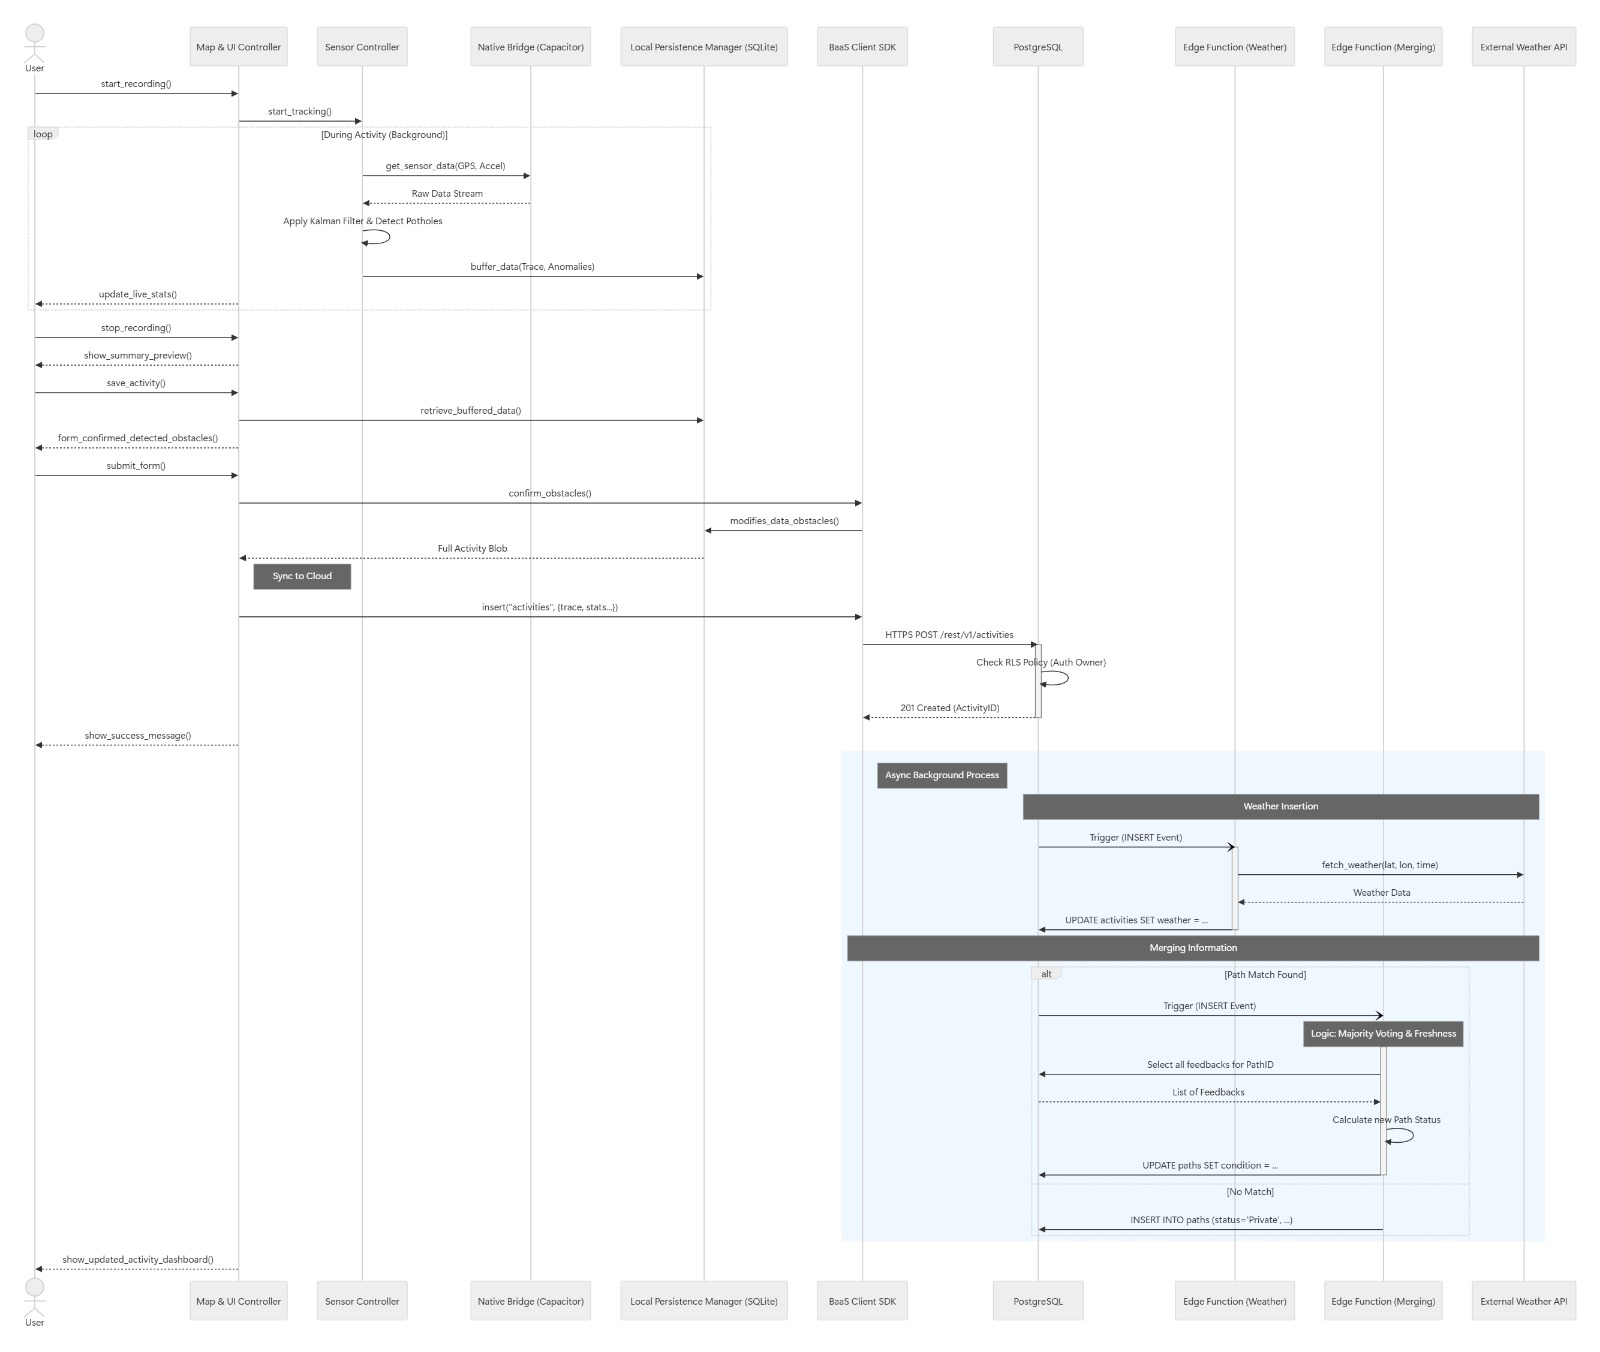
\includegraphics[width=\textwidth]{Images/uc3_sd.jpeg}
    \caption{[UC3] Activity Recording Sequence Diagram}
    \label{fig:sd_uc3}
\end{figure}
The diagram highlights the Thick Client and Offline-First architecture. Data acquisition is performed via the Native Bridge, filtered, and saved locally on SQLite. Synchronization with the Cloud triggers asynchronous processes (Serverless): meteorological enrichment and the Merging logic. Note that the trace comparison logic occurs entirely server-side (Edge Function) to avoid burdening the user device and to guarantee data consistency.

% --- UC4: Creation of a manual path ---
\subsubsection*{[UC4] Creation of a manual path Sequence Diagram}
\begin{figure}[H]
    \centering
    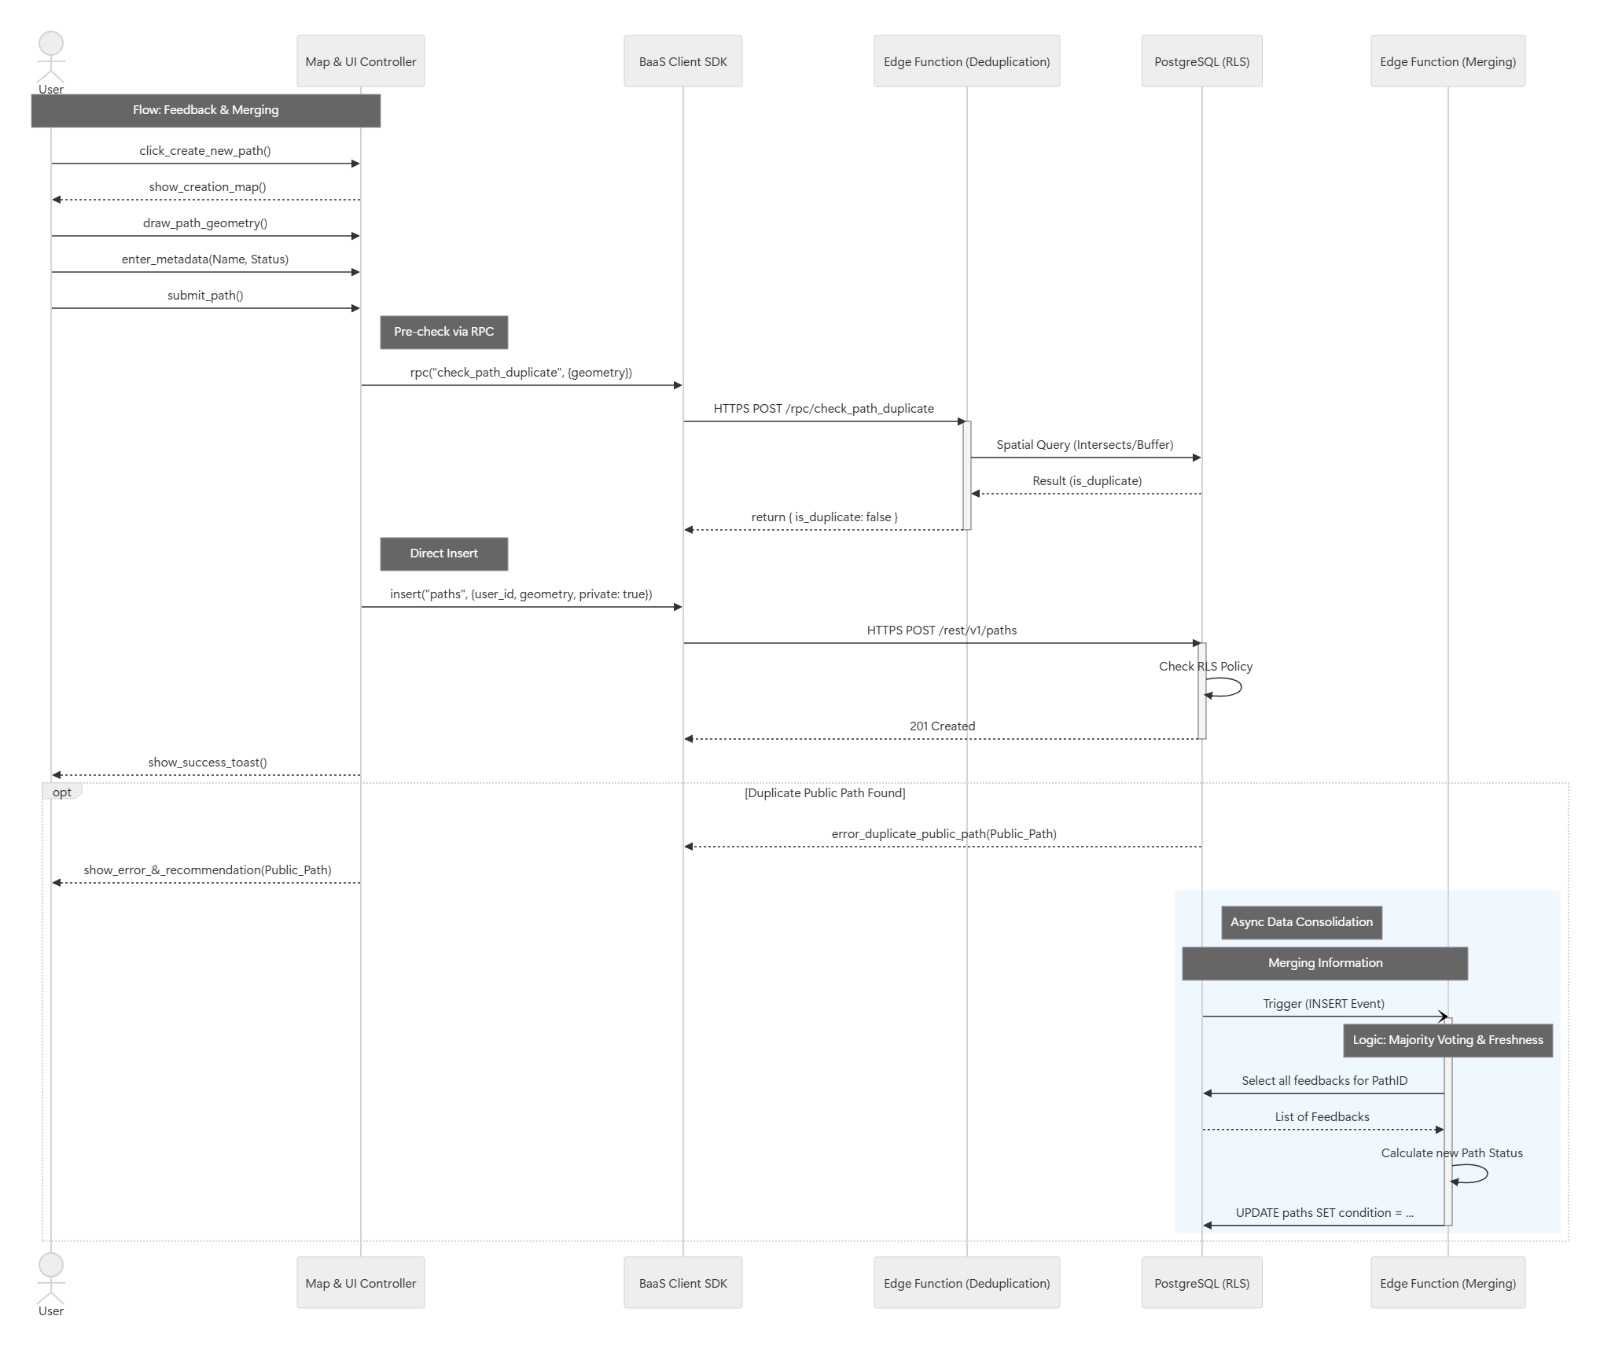
\includegraphics[width=\textwidth]{Images/uc4_sd.jpeg}
    \caption{[UC4] Creation of a manual path Sequence Diagram}
    \label{fig:sd_uc4}
\end{figure}
This scenario illustrates the hybrid interaction between direct DB calls and server-side logic. Before inserting the path, the client invokes a Remote Procedure Call (RPC) on a specific Edge Function (Deduplication) to verify the existence of duplicate paths via complex spatial queries (PostGIS). If the check passes, the client proceeds with direct insertion into the database; otherwise, it merges the information entered by the user into the existing public path that corresponds to the inserted geometry.

% --- UC5: Publication of a path ---
\subsubsection*{[UC5] Publication of a path Sequence Diagram}
\begin{figure}[H]
    \centering
    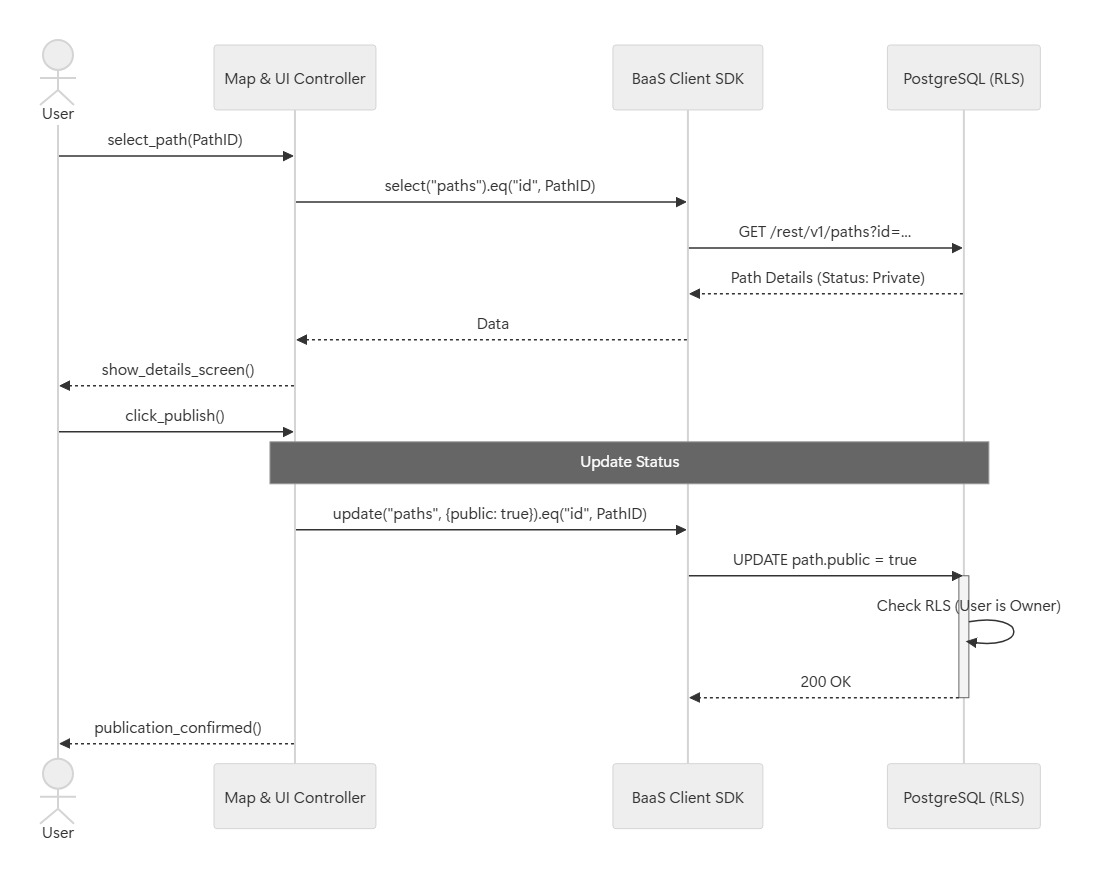
\includegraphics[width=\textwidth]{Images/uc5_sd.jpeg}
    \caption{[UC5] Publication of a path Sequence Diagram}
    \label{fig:sd_uc5}
\end{figure}
This represents the state transition of a path from Private to Public. The operation is a direct UPDATE call via the SDK. Security is guaranteed by the PostgreSQL database engine, which, through RLS policies, verifies that the request author corresponds to the record owner before applying the modification.

% --- UC6: Path Feedback reporting ---
\subsubsection*{[UC6] Path Feedback reporting Sequence Diagram}
\begin{figure}[H]
    \centering
    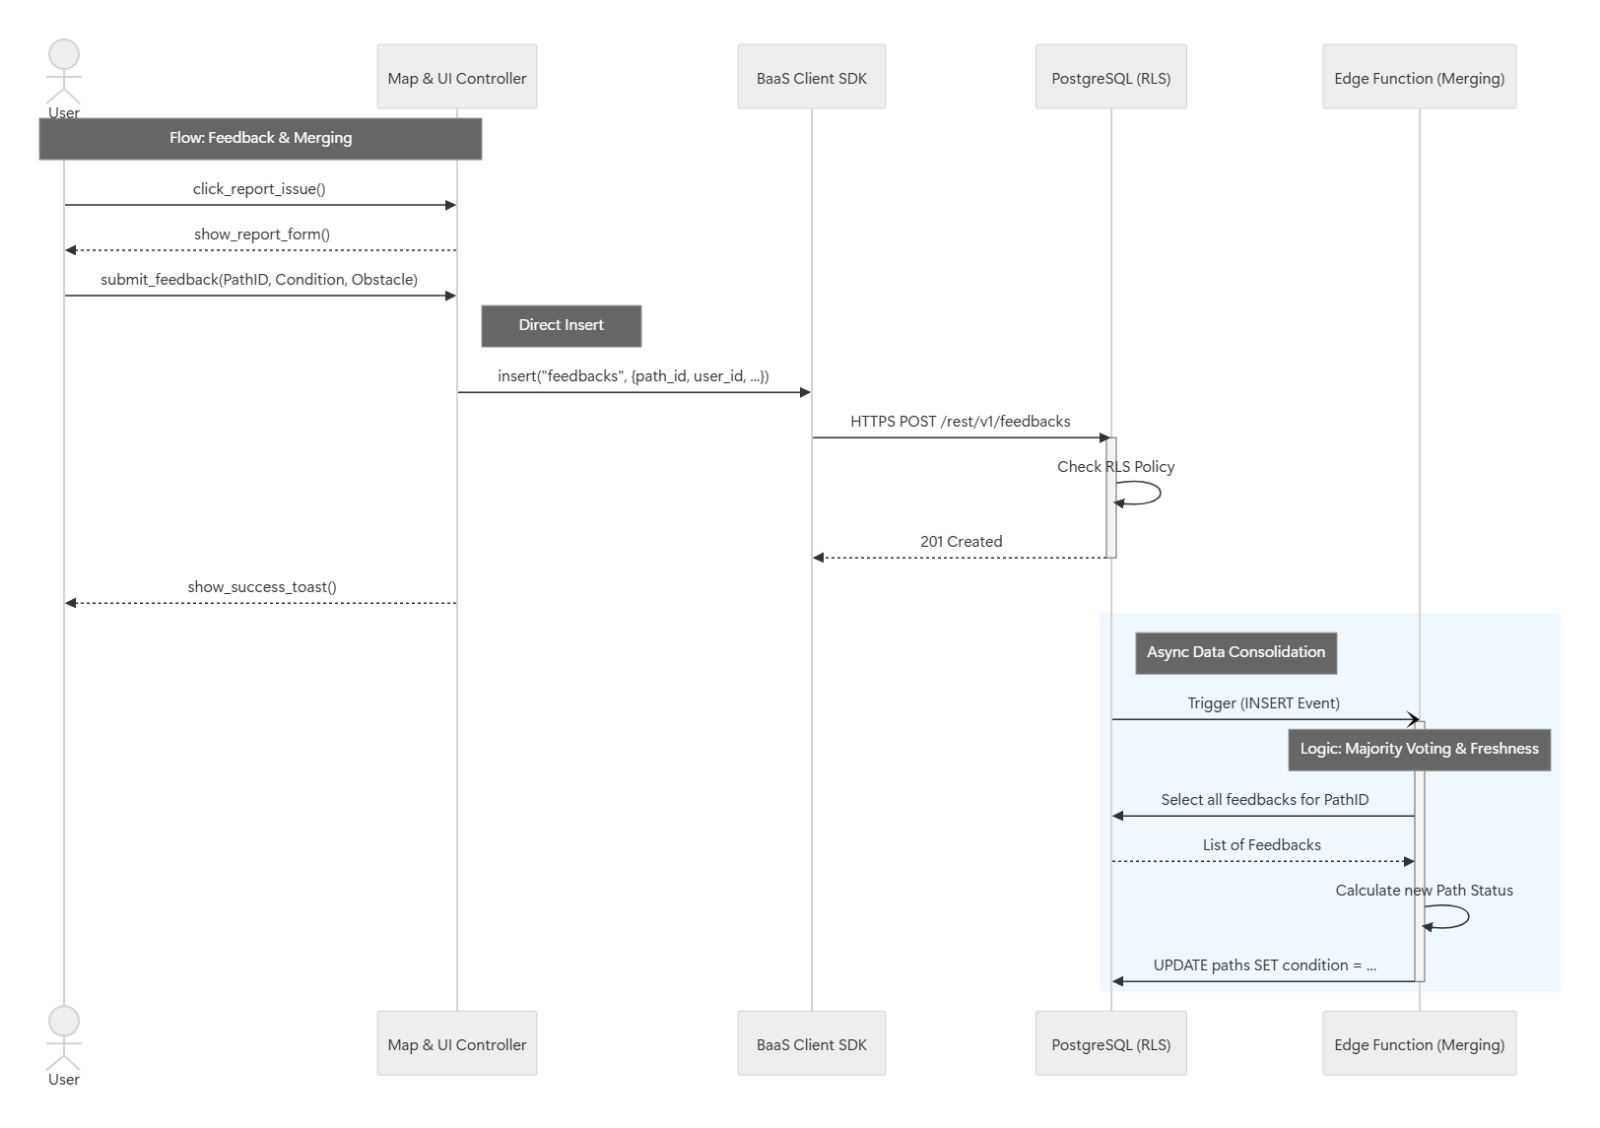
\includegraphics[width=\textwidth]{Images/uc6_sd.jpeg}
    \caption{[UC6] Path Feedback reporting Sequence Diagram}
    \label{fig:sd_uc6}
\end{figure}
The diagram demonstrates the Event-Driven architecture. The client handles only the rapid insertion of the feedback to ensure user responsiveness. The database emits an internal event (Trigger) that asynchronously activates the Merging Edge Function. This function recalculates the path status by aggregating existing feedbacks according to the "Majority Voting" algorithm defined in the RASD.

% --- UC7: Search for a path ---
\subsubsection*{[UC7] Search for a path Sequence Diagram}
\begin{figure}[H]
    \centering
    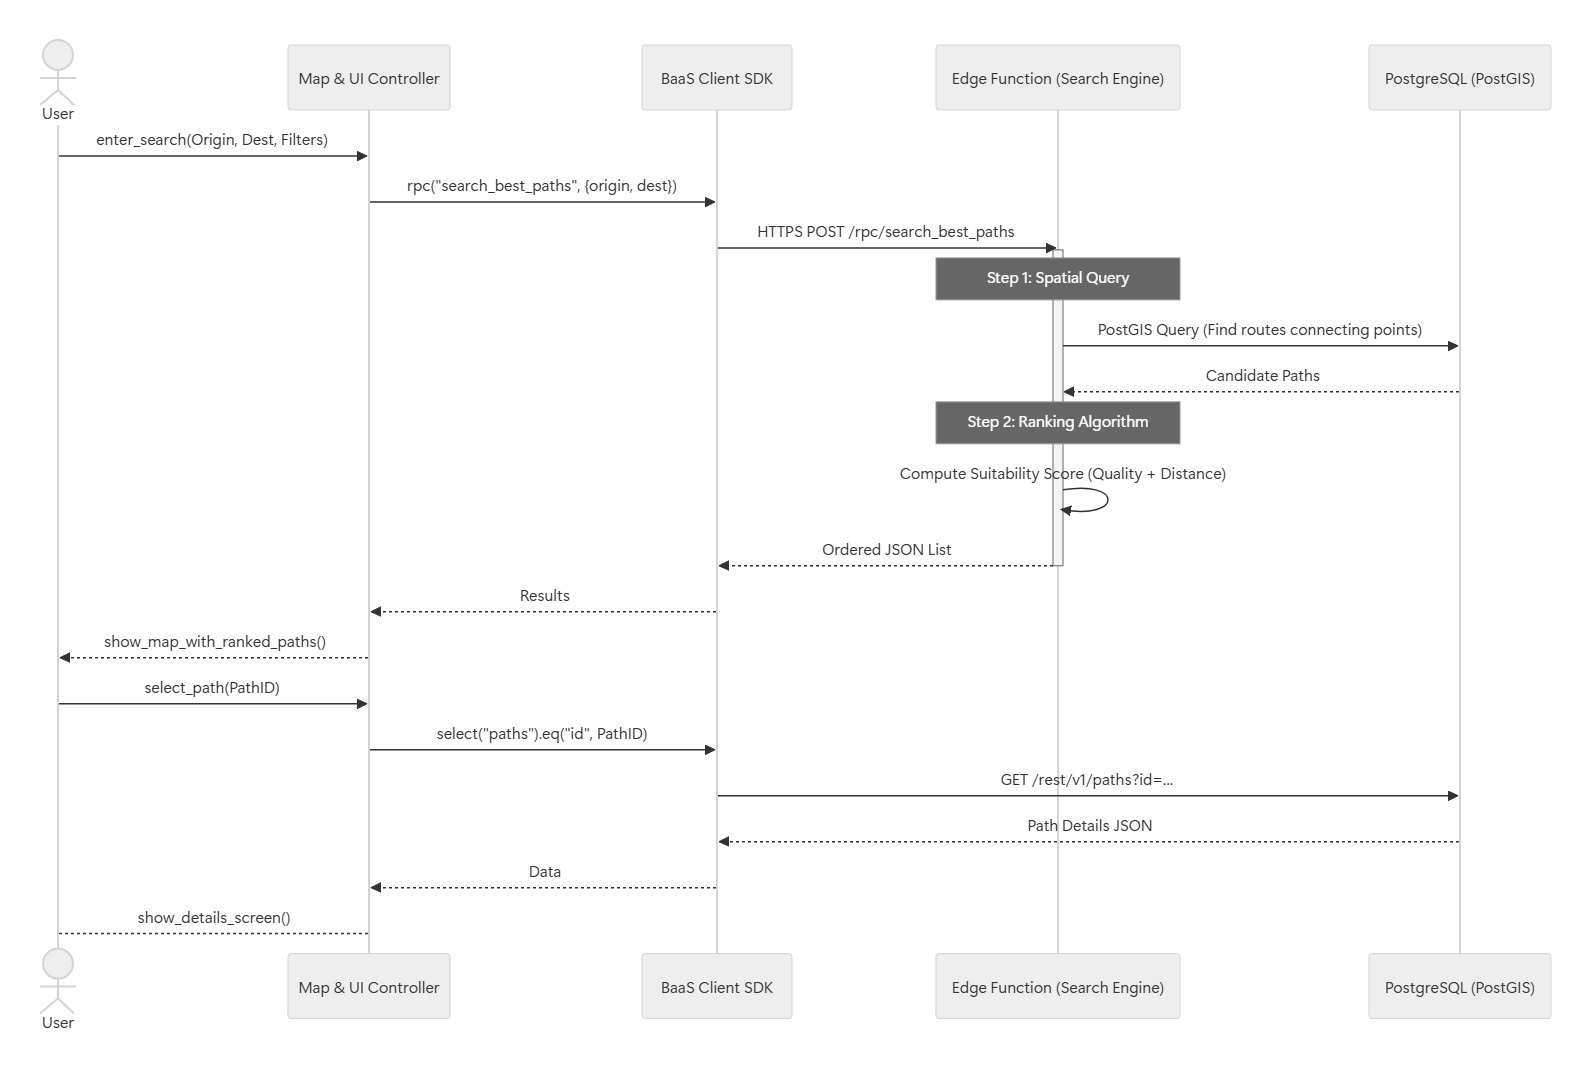
\includegraphics[width=\textwidth]{Images/uc7_sd.jpeg}
    \caption{[UC7] Search for a path Sequence Diagram}
    \label{fig:sd_uc7}
\end{figure}
Since the ranking algorithm requires complex calculations (combining geometric distance and quality score), the search is not a simple DB query but is encapsulated in an RPC (Remote Procedure Call). The Edge Function executes the spatial query on PostGIS and sorts the results in memory before returning them to the client, optimizing performance and reducing data traffic.

\section{Component interfaces}
This section specifies the APIs provided and required by the major components identified in the Component View. The interfaces are categorized into \textbf{Hardware Abstraction Interfaces} (internal to the Hybrid Client) and \textbf{Network Interfaces} (between Client and Cloud).

\subsection{Hardware Abstraction Interfaces}
These interfaces are exposed by the \textbf{Native Bridge (Capacitor)} and consumed by the \textbf{Sensor Controller} component within the web runtime. They allow the TypeScript application logic to access device sensors.

\paragraph{Interface: IGeolocationProvider}
\begin{itemize}
    \item \textbf{Description:} Provides access to the device's GPS hardware.
    \item \textbf{Provided By:} Native Bridge (\texttt{@capacitor/geolocation})
    \item \textbf{Used By:} Sensor Controller
\end{itemize}

\begin{table}[H]
\centering
\renewcommand{\arraystretch}{1.4}
\begin{tabular}{|p{0.22\textwidth}|p{0.25\textwidth}|p{0.18\textwidth}|p{0.25\textwidth}|}
\hline
\textbf{Method Signature} & \textbf{Input Parameters} & \textbf{Return Value} & \textbf{Description} \\
\hline
\texttt{getCurrentPosition()} & \texttt{options: GeoOptions} & \texttt{Promise<Position>} & Returns the single current coordinate (Lat, Long, Altitude). \\
\hline
\texttt{watchPosition()} & \texttt{options: GeoOptions, callback: (pos) => void} & \texttt{CallbackID} & Starts a continuous background location tracking session. The callback is invoked every time the OS receives a location update. \\
\hline
\texttt{clearWatch()} & \texttt{id: CallbackID} & \texttt{void} & Stops the tracking session to save battery. \\
\hline
\end{tabular}
\caption{IGeolocationProvider Interface}
\end{table}

\paragraph{Interface: IMotionSensor}
\begin{itemize}
    \item \textbf{Description:} Provides high-frequency access to the accelerometer for pothole detection.
    \item \textbf{Provided By:} Native Bridge (\texttt{@capacitor/motion})
    \item \textbf{Used By:} Sensor Controller (Inertial Analyzer)
\end{itemize}

\begin{table}[H]
\centering
\renewcommand{\arraystretch}{1.4}
\begin{tabular}{|p{0.22\textwidth}|p{0.25\textwidth}|p{0.18\textwidth}|p{0.25\textwidth}|}
\hline
\textbf{Method Signature} & \textbf{Input Parameters} & \textbf{Return Value} & \textbf{Description} \\
\hline
\texttt{addListener()} & \texttt{eventName: 'accel', callback: (event) => void} & \texttt{PluginListenerHandle} & Subscribes to the raw accelerometer stream. The event contains $x, y, z$ acceleration vectors used to detect vertical shocks. \\
\hline
\texttt{removeAllListeners()} & \texttt{void} & \texttt{void} & Unsubscribes from the sensor stream. \\
\hline
\end{tabular}
\caption{IMotionSensor Interface}
\end{table}

\subsection{Cloud Network Interfaces (BaaS API)}
These interfaces represent the communication contract between the \textbf{Hybrid Client} and the \textbf{Serverless Cloud}. Since the architecture uses a BaaS, these are primarily RESTful endpoints automatically generated by Supabase from the database schema, plus RPC (Remote Procedure Calls) for Edge Functions.

\paragraph{Interface: IAuthService}
\begin{itemize}
    \item \textbf{Description:} Manages user sessions.
    \item \textbf{Protocol:} HTTPS / REST
    \item \textbf{Provided By:} Auth Service (Supabase GoTrue)
\end{itemize}

\begin{table}[H]
\centering
\renewcommand{\arraystretch}{1.4}
\begin{tabular}{|p{0.25\textwidth}|p{0.25\textwidth}|p{0.20\textwidth}|p{0.20\textwidth}|}
\hline
\textbf{Endpoint / Method} & \textbf{Input Payload} & \textbf{Response} & \textbf{Description} \\
\hline
\texttt{POST /auth/v1/signup} & \texttt{\{ email, password \}} & \texttt{\{ user, session, jwt \}} & Registers a new user and returns the access token. \\
\hline
\texttt{POST /auth/v1/token} & \texttt{\{ email, password, grant\_type \}} & \texttt{\{ access\_token, refresh\_token \}} & Authenticates a user (Login). \\
\hline
\texttt{POST /auth/v1/logout} & Header: \texttt{Bearer <token>} & \texttt{204 No Content} & Invalidates the current session. \\
\hline
\end{tabular}
\caption{IAuthService Interface}
\end{table}

\paragraph{Interface: ISpatialDataStore}
\begin{itemize}
    \item \textbf{Description:} Provides CRUD access to geospatial entities. Access is filtered by RLS policies.
    \item \textbf{Protocol:} HTTPS / REST
    \item \textbf{Provided By:} Spatial Database (PostgREST)
\end{itemize}

\begin{table}[H]
\centering
\renewcommand{\arraystretch}{1.4}
\begin{tabular}{|p{0.25\textwidth}|p{0.25\textwidth}|p{0.20\textwidth}|p{0.20\textwidth}|}
\hline
\textbf{Endpoint / Method} & \textbf{Input Payload} & \textbf{Response} & \textbf{Description} \\
\hline
\texttt{GET /rest/v1/paths} & Query Params: \texttt{select=*, geometry=...} & \texttt{JSON Array} & Retrieves public paths. Supports spatial filtering (e.g., retrieving paths within a map viewport). \\
\hline
\texttt{POST /rest/v1/activities} & \texttt{\{ user\_id, geometry\_linestring, ... \}} & \texttt{201 Created} & Uploads a recorded activity trace. This action triggers the \texttt{func\_path\_merging} Edge Function asynchronously. \\
\hline
\texttt{POST /rest/v1/feedbacks} & \texttt{\{ path\_id, rating, comment \}} & \texttt{201 Created} & Submits a user report for a specific path. \\
\hline
\end{tabular}
\caption{ISpatialDataStore Interface}
\end{table}

\paragraph{Interface: ISearchEngine (RPC)}
\begin{itemize}
    \item \textbf{Description:} Exposes the complex path ranking logic as a remote function call.
    \item \textbf{Protocol:} HTTPS / RPC
    \item \textbf{Provided By:} Edge Functions
\end{itemize}

\begin{table}[H]
\centering
\renewcommand{\arraystretch}{1.4}
\begin{tabular}{|p{0.25\textwidth}|p{0.25\textwidth}|p{0.20\textwidth}|p{0.20\textwidth}|}
\hline
\textbf{Function Name} & \textbf{Input Parameters} & \textbf{Return Value} & \textbf{Description} \\
\hline
\texttt{rpc/search\_best\_paths} & \texttt{\{ origin\_lat, origin\_lon, dest\_lat, dest\_lon \}} & \texttt{JSON Array <Path>} & Invokes the routing algorithm. Returns a list of paths ordered by the dynamic \textbf{Suitability Score} (calculated based on distance and road quality). \\
\hline
\end{tabular}
\caption{ISearchEngine Interface}
\end{table}

\subsection{External Interfaces}

\paragraph{Interface: IWeatherProvider}
\begin{itemize}
    \item \textbf{Description:} External API used to enrich path data with meteorological conditions.
    \item \textbf{Provided By:} Third-party provider (e.g., OpenWeatherMap)
    \item \textbf{Used By:} \texttt{func\_weather\_enricher} (Edge Function)
\end{itemize}

\begin{table}[H]
\centering
\renewcommand{\arraystretch}{1.4}
\begin{tabular}{|p{0.25\textwidth}|p{0.15\textwidth}|p{0.20\textwidth}|p{0.30\textwidth}|}
\hline
\textbf{Endpoint} & \textbf{Method} & \textbf{Params} & \textbf{Description} \\
\hline
\texttt{/data/2.5/weather} & \texttt{GET} & \texttt{lat, lon, appid} & Fetches current weather data (Temperature, Rain volume, Wind) for a specific coordinate. \\
\hline
\end{tabular}
\caption{IWeatherProvider Interface}
\end{table}
\section{Selected architectural styles and patterns}
\subsection{Architectural Styles}

\begin{itemize}
    \item \textbf{Serverless / Backend-as-a-Service (BaaS)}
    \begin{itemize}
        \item \textbf{Description:} The system does not rely on a traditional, self-managed monolithic application server. Instead, backend responsibilities, including database management, authentication, and file storage, are delegated to a managed cloud provider (Supabase). Application logic is executed via stateless containers (Edge Functions) that spin up only when triggered.
        \item \textbf{Rationale:} This style was chosen to maximize scalability and minimize operational overhead. Since the "Best Bike Paths" system must handle potential spikes in usage without manual provisioning, a serverless infrastructure ensures automatic scaling. Furthermore, it allows the development team to focus entirely on the complex domain logic (merging and ranking) rather than server maintenance and patching.
    \end{itemize}

    \item \textbf{Event-Driven Architecture}
    \begin{itemize}
        \item \textbf{Description:} The interaction between data ingestion and data processing is decoupled. When a client uploads a new activity, the system does not process it synchronously. Instead, the database emits an event (webhook), which asynchronously triggers the specific Edge Function responsible for the merging algorithm.
        \item \textbf{Rationale:} The Path Merging process involves complex geospatial calculations (intersections, buffering) that are computationally expensive. Processing them synchronously would block the client UI and lead to connection timeouts. An event-driven approach ensures the user interface remains responsive (Latency Hiding) while heavy tasks are processed in the background.
    \end{itemize}

    \item \textbf{Thick Client}
    \begin{itemize}
        \item \textbf{Description:} A significant portion of the application logic resides on the client device rather than the server. The Hybrid Client is responsible for sensor data acquisition, noise filtering (Kalman Filter), data validation, and local buffering.
        \item \textbf{Rationale:} This style is strictly required to satisfy the reliability constraints defined in the RASD. Cyclists often traverse areas with no network coverage; the client must be able to function autonomously, recording and validating data locally, and syncing only when connectivity is restored.
    \end{itemize}
\end{itemize}

\subsection{Design Patterns}

\begin{itemize}
    \item \textbf{Bridge Pattern (via Capacitor)}
    \begin{itemize}
        \item \textbf{Description:} The application utilizes a native bridge to decouple the high-level application logic (written in TypeScript/React) from the low-level platform implementation (Android/iOS). The web code calls a uniform JavaScript API, and the Bridge translates these calls into native OS commands.
        \item \textbf{Rationale:} This pattern enables cross-platform accessibility while satisfying the need for hardware-specific features. Specifically, Capacitor native plugins allows the web-based application to access the accelerometer and background geolocation services, which are otherwise inaccessible or limited in a standard browser environment.
    \end{itemize}

    \item \textbf{Observer Pattern}
    \begin{itemize}
        \item \textbf{Description:} The client application subscribes to real-time changes on specific database tables (e.g., \texttt{Feedbacks}) using Secure WebSockets (WSS). When the data changes on the server, the new state is automatically pushed to all listening clients.
        \item \textbf{Rationale:} This is essential for the safety-critical feature of reporting road hazards. If a user reports a danger, other nearby cyclists must be notified immediately to update their map view, without needing to manually refresh the application.
    \end{itemize}

    \item \textbf{Row Level Security (RLS)}
    \begin{itemize}
        \item \textbf{Description:} Access control logic is implemented directly within the database engine rather than in the application code. Each database query is evaluated against a set of SQL policies that check the user's authentication token against the data being accessed.
        \item \textbf{Rationale:} Since the architecture allows clients to communicate directly with the database (skipping the middleware layer), RLS is the only mechanism to guarantee data isolation. It mathematically ensures that a user can never read or modify another user's private data, regardless of any potential bug in the client code.
    \end{itemize}
\end{itemize}
\section{Other design decisions}
\subsection{Adoption of Hybrid Mobile Architecture}
\begin{itemize}
    \item \textbf{Description:} The development strategy involves building a single web-based codebase wrapped in a native container (Capacitor), rather than developing two separate native applications (Kotlin for Android, Swift for iOS) or a pure Progressive Web App (PWA).
    \item \textbf{Rationale:} A pure PWA was discarded because it cannot reliably access high-frequency motion sensors in the background, which is critical for the "Road Quality Detection" requirement. Native development was discarded due to the high effort required for a small team. The Hybrid approach offers the necessary hardware access with a unified codebase, significantly reducing development and testing time.
\end{itemize}

\subsection{Usage of PostgreSQL with PostGIS}
\begin{itemize}
    \item \textbf{Description:} The system utilizes a Relational Database Management System (RDBMS) extended with the PostGIS spatial engine to store and query all geospatial data (Points, Linestrings, Polygons).
    \item \textbf{Rationale:} Generic databases are insufficient for the mathematical complexity of this project. PostGIS provides native, highly optimized functions for geospatial conflation and Nearest-Neighbor searches. Implementing these geometric algorithms from scratch in code would be error-prone and inefficient.
\end{itemize}

\subsection{Centralized Logic for Merging and Ranking}
\begin{itemize}
    \item \textbf{Description:} The core algorithms that determine the shape of public paths (Merging) and their value (Ranking) are executed exclusively on the Cloud Tier via Edge Functions, never on the client.
    \item \textbf{Rationale:} This decision ensures a \textbf{Single Source of Truth}. The merging algorithm requires a complete view of all existing paths in an area to make a decision, which a single client does not possess. Furthermore, calculating the Ranking on the server prevents malicious users from tampering with the client code to artificially inflate the score of their preferred paths.
\end{itemize}

\subsection{Direct-to-Database Communication Pattern}
\begin{itemize}
    \item \textbf{Description:} The architecture bypasses the traditional "API Gateway / Controller" layer for standard operations. Clients perform CRUD (Create, Read, Update, Delete) operations directly against the database's REST API.
    \item \textbf{Rationale:} The majority of user interactions (e.g., loading a profile, saving a track) are standard data operations that do not require complex business logic. Implementing a dedicated middle-layer for these simple tasks would introduce unnecessary latency and code maintenance ("Boilerplate"). Security is delegated to RLS (as described in 2.6.2), making the middle layer redundant for these tasks.
\end{itemize}

%------------------------------------------------------------------------------------------------------------------------------------------------
\clearpage
\chapter{{User Interface Design}}
\label{sect:user_interface_design}

This section outlines the main user interface views and the rationale behind their layout. Each screen is described with its \textbf{primary goals}, \textbf{key interactions}, and \textbf{visual hierarchy} choices to ensure quick comprehension, consistency across flows, and usability in both \textbf{desktop} and \textbf{mobile} contexts.

\begin{figure}[H]
	\centering
	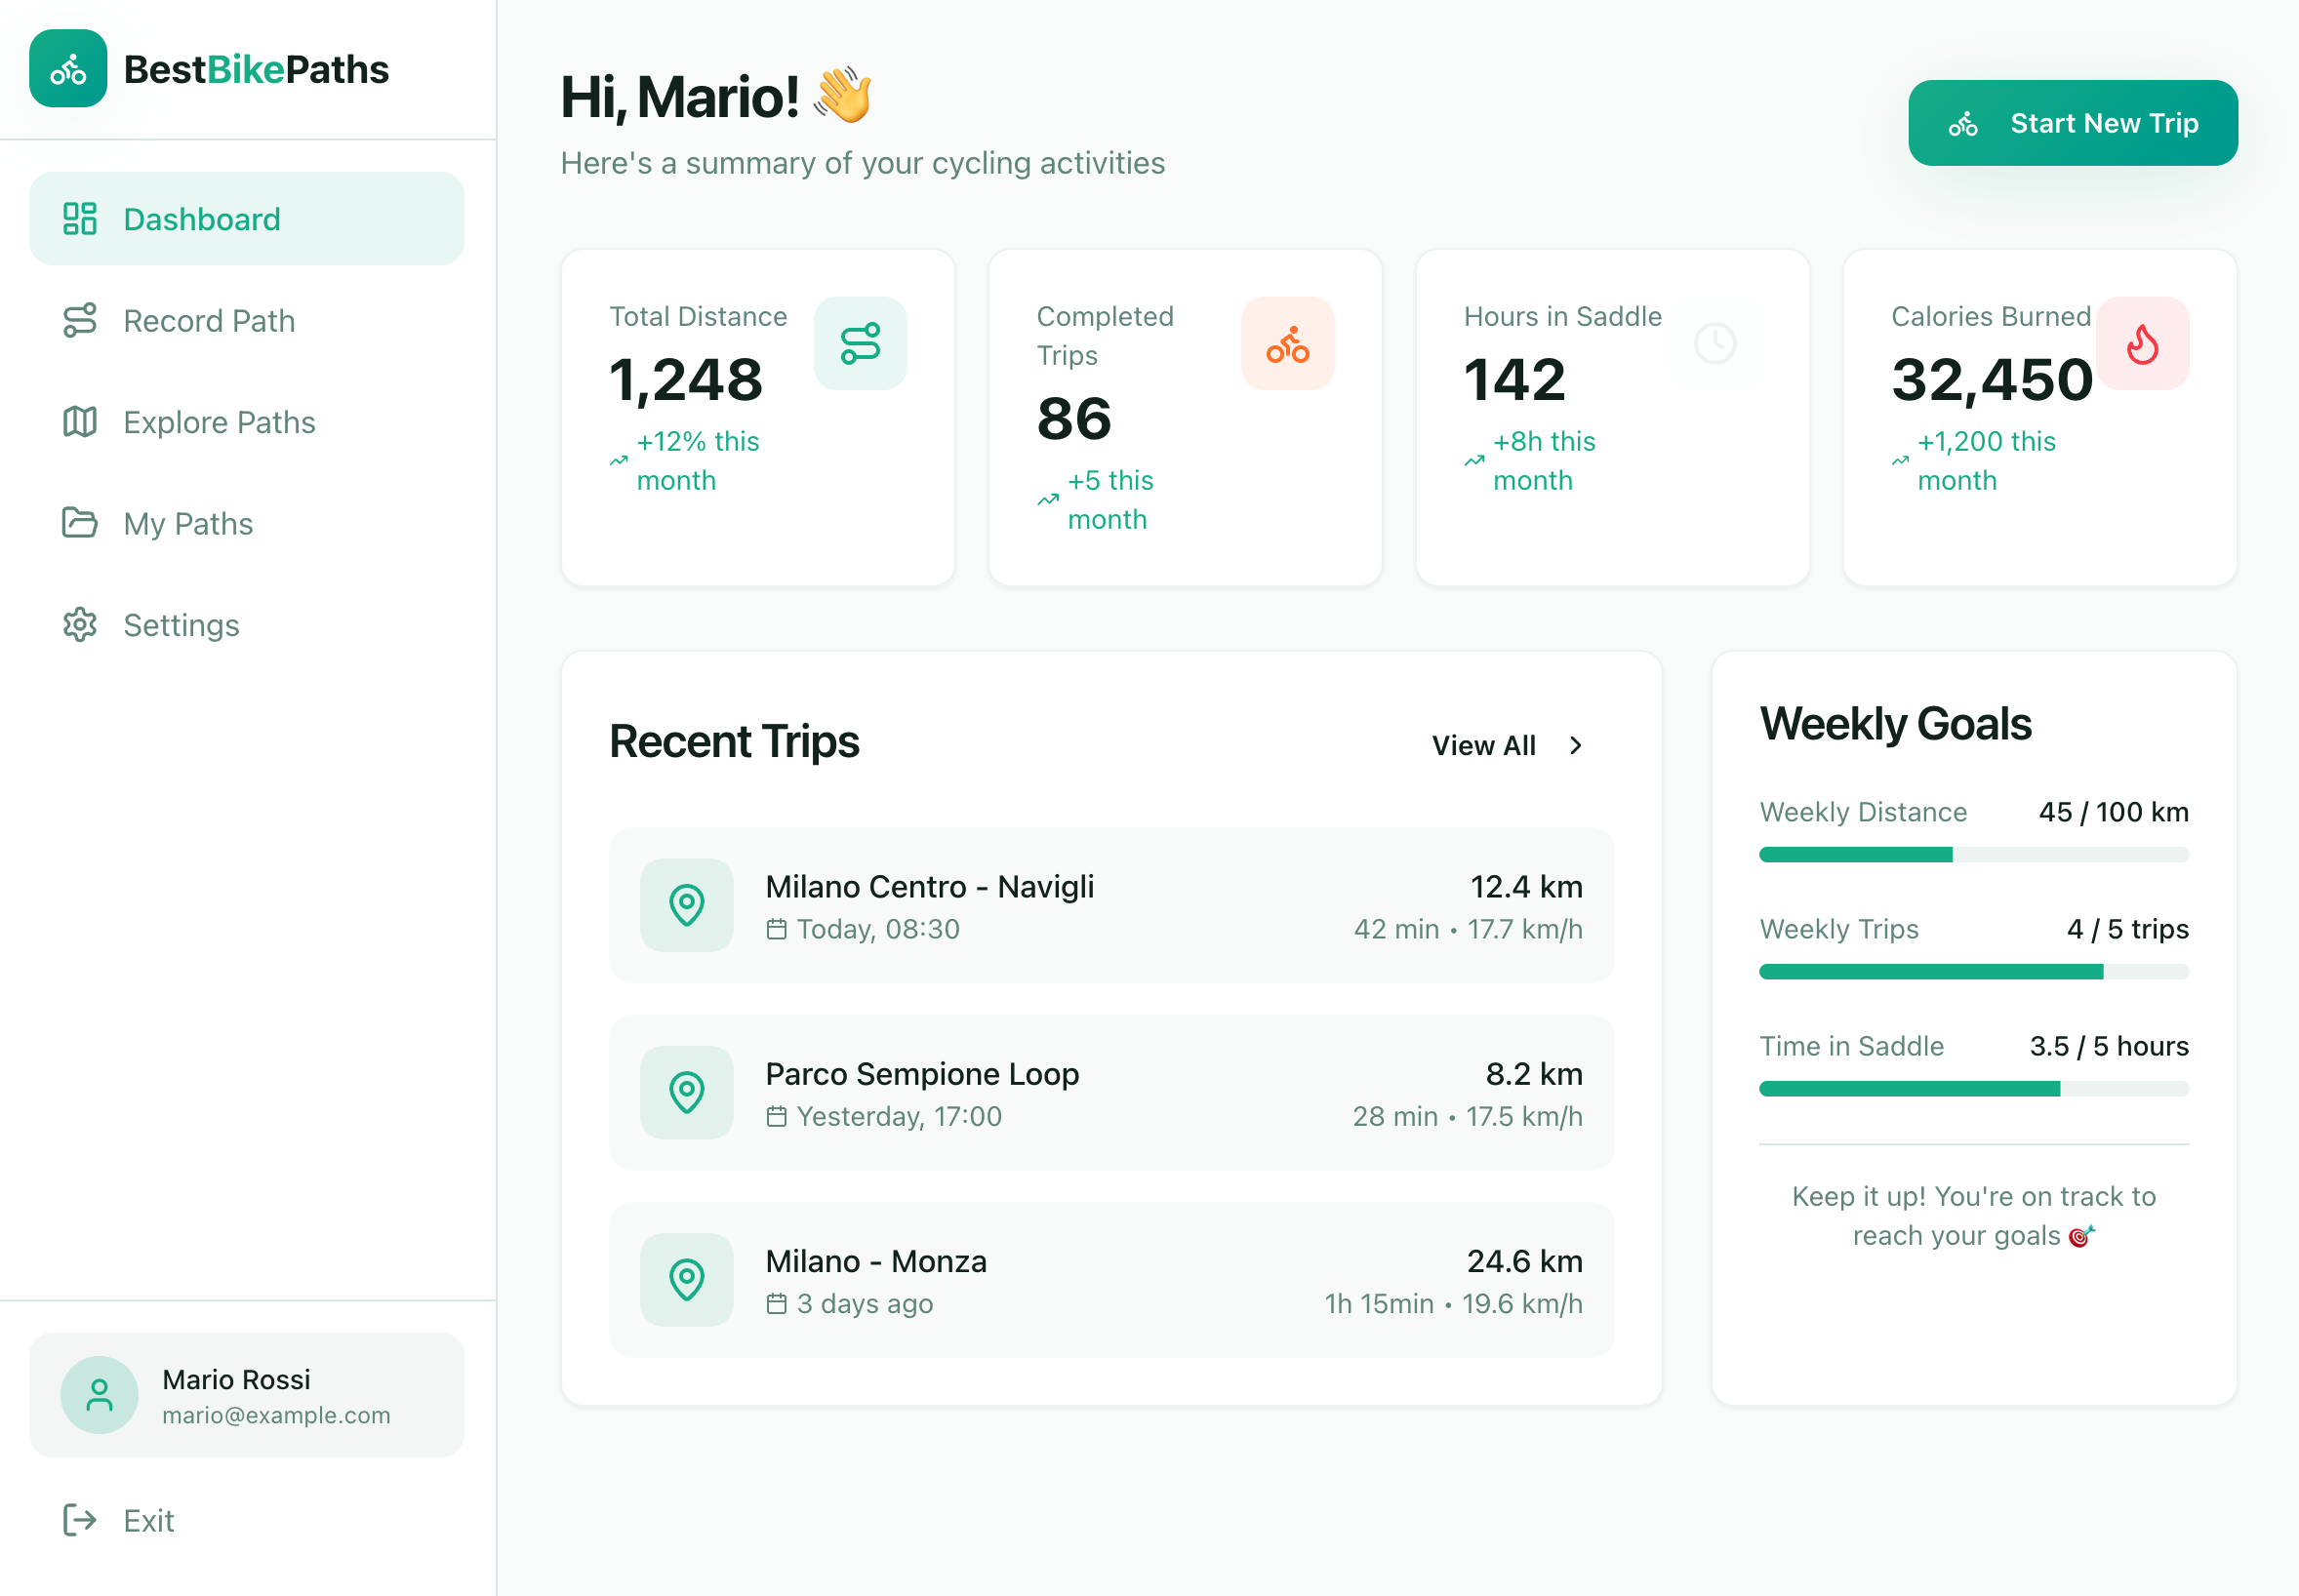
\includegraphics[width=0.8\textwidth]{Images/dashboard.png}
	\caption{Main dashboard summarizing service status, recent notifications, and quick actions.}
	\label{fig:dashboard}
\end{figure}

The \textbf{dashboard} provides an immediate summary of the most relevant information: \textbf{active services status}, \textbf{recent notifications}, \textbf{shortcuts} to the most frequent actions, and compact \textbf{trend charts}. Content is organized in \textbf{cards} to allow fast scanning and \textbf{responsive} flow; each card highlights the primary \textbf{KPI} or status and, when relevant, a \textbf{trend indicator}. A \textbf{left navigation bar} leads to the operational sections, while the \textbf{header} shows the name of the user and a button to \textbf{record a new activity}.

\begin{figure}[H]
	\centering
	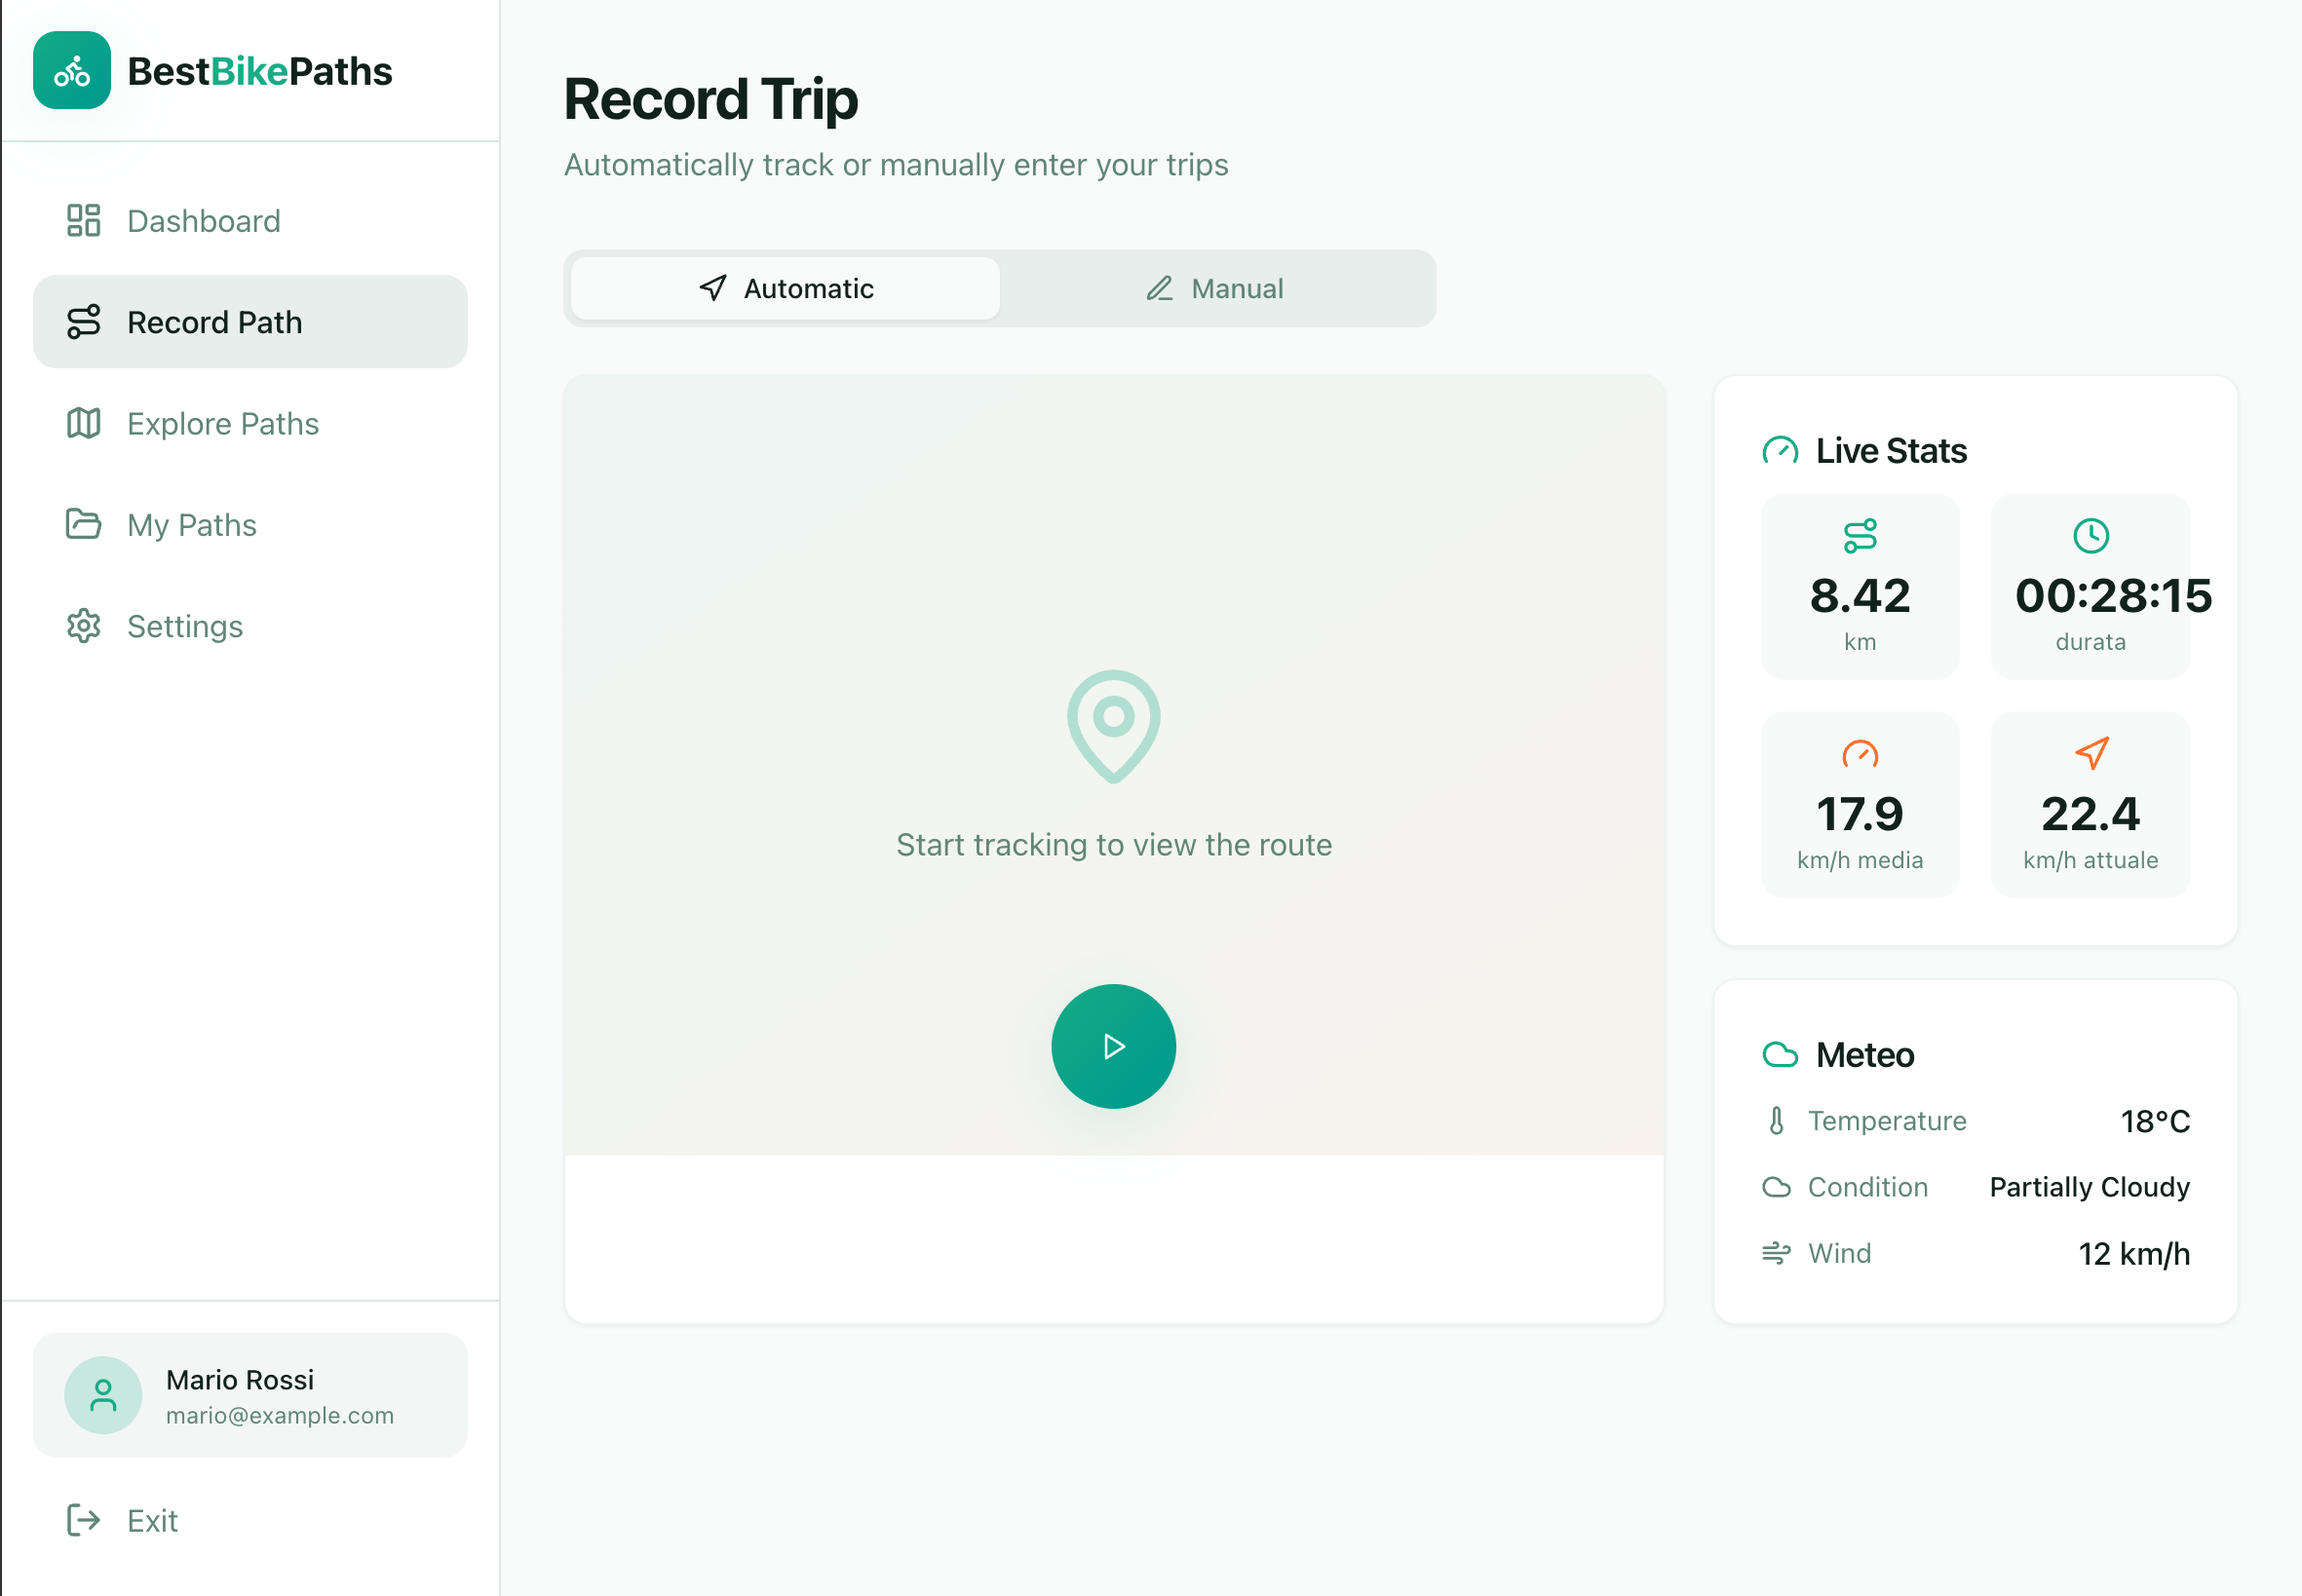
\includegraphics[width=0.8\textwidth]{Images/registra_viaggio.png}
	\caption{Trip recording interface with live metrics and waypoint controls.}
	\label{fig:registra-viaggio}
\end{figure}
The recording screen foregrounds the \textbf{start/stop control} and \textbf{live metrics} (\textbf{distance}, \textbf{duration}, \textbf{pace}). Secondary actions allow adding \textbf{waypoints} or \textbf{notes}; the layout keeps high \textbf{contrast} for outdoor readability.

\begin{figure}[H]
	\centering
	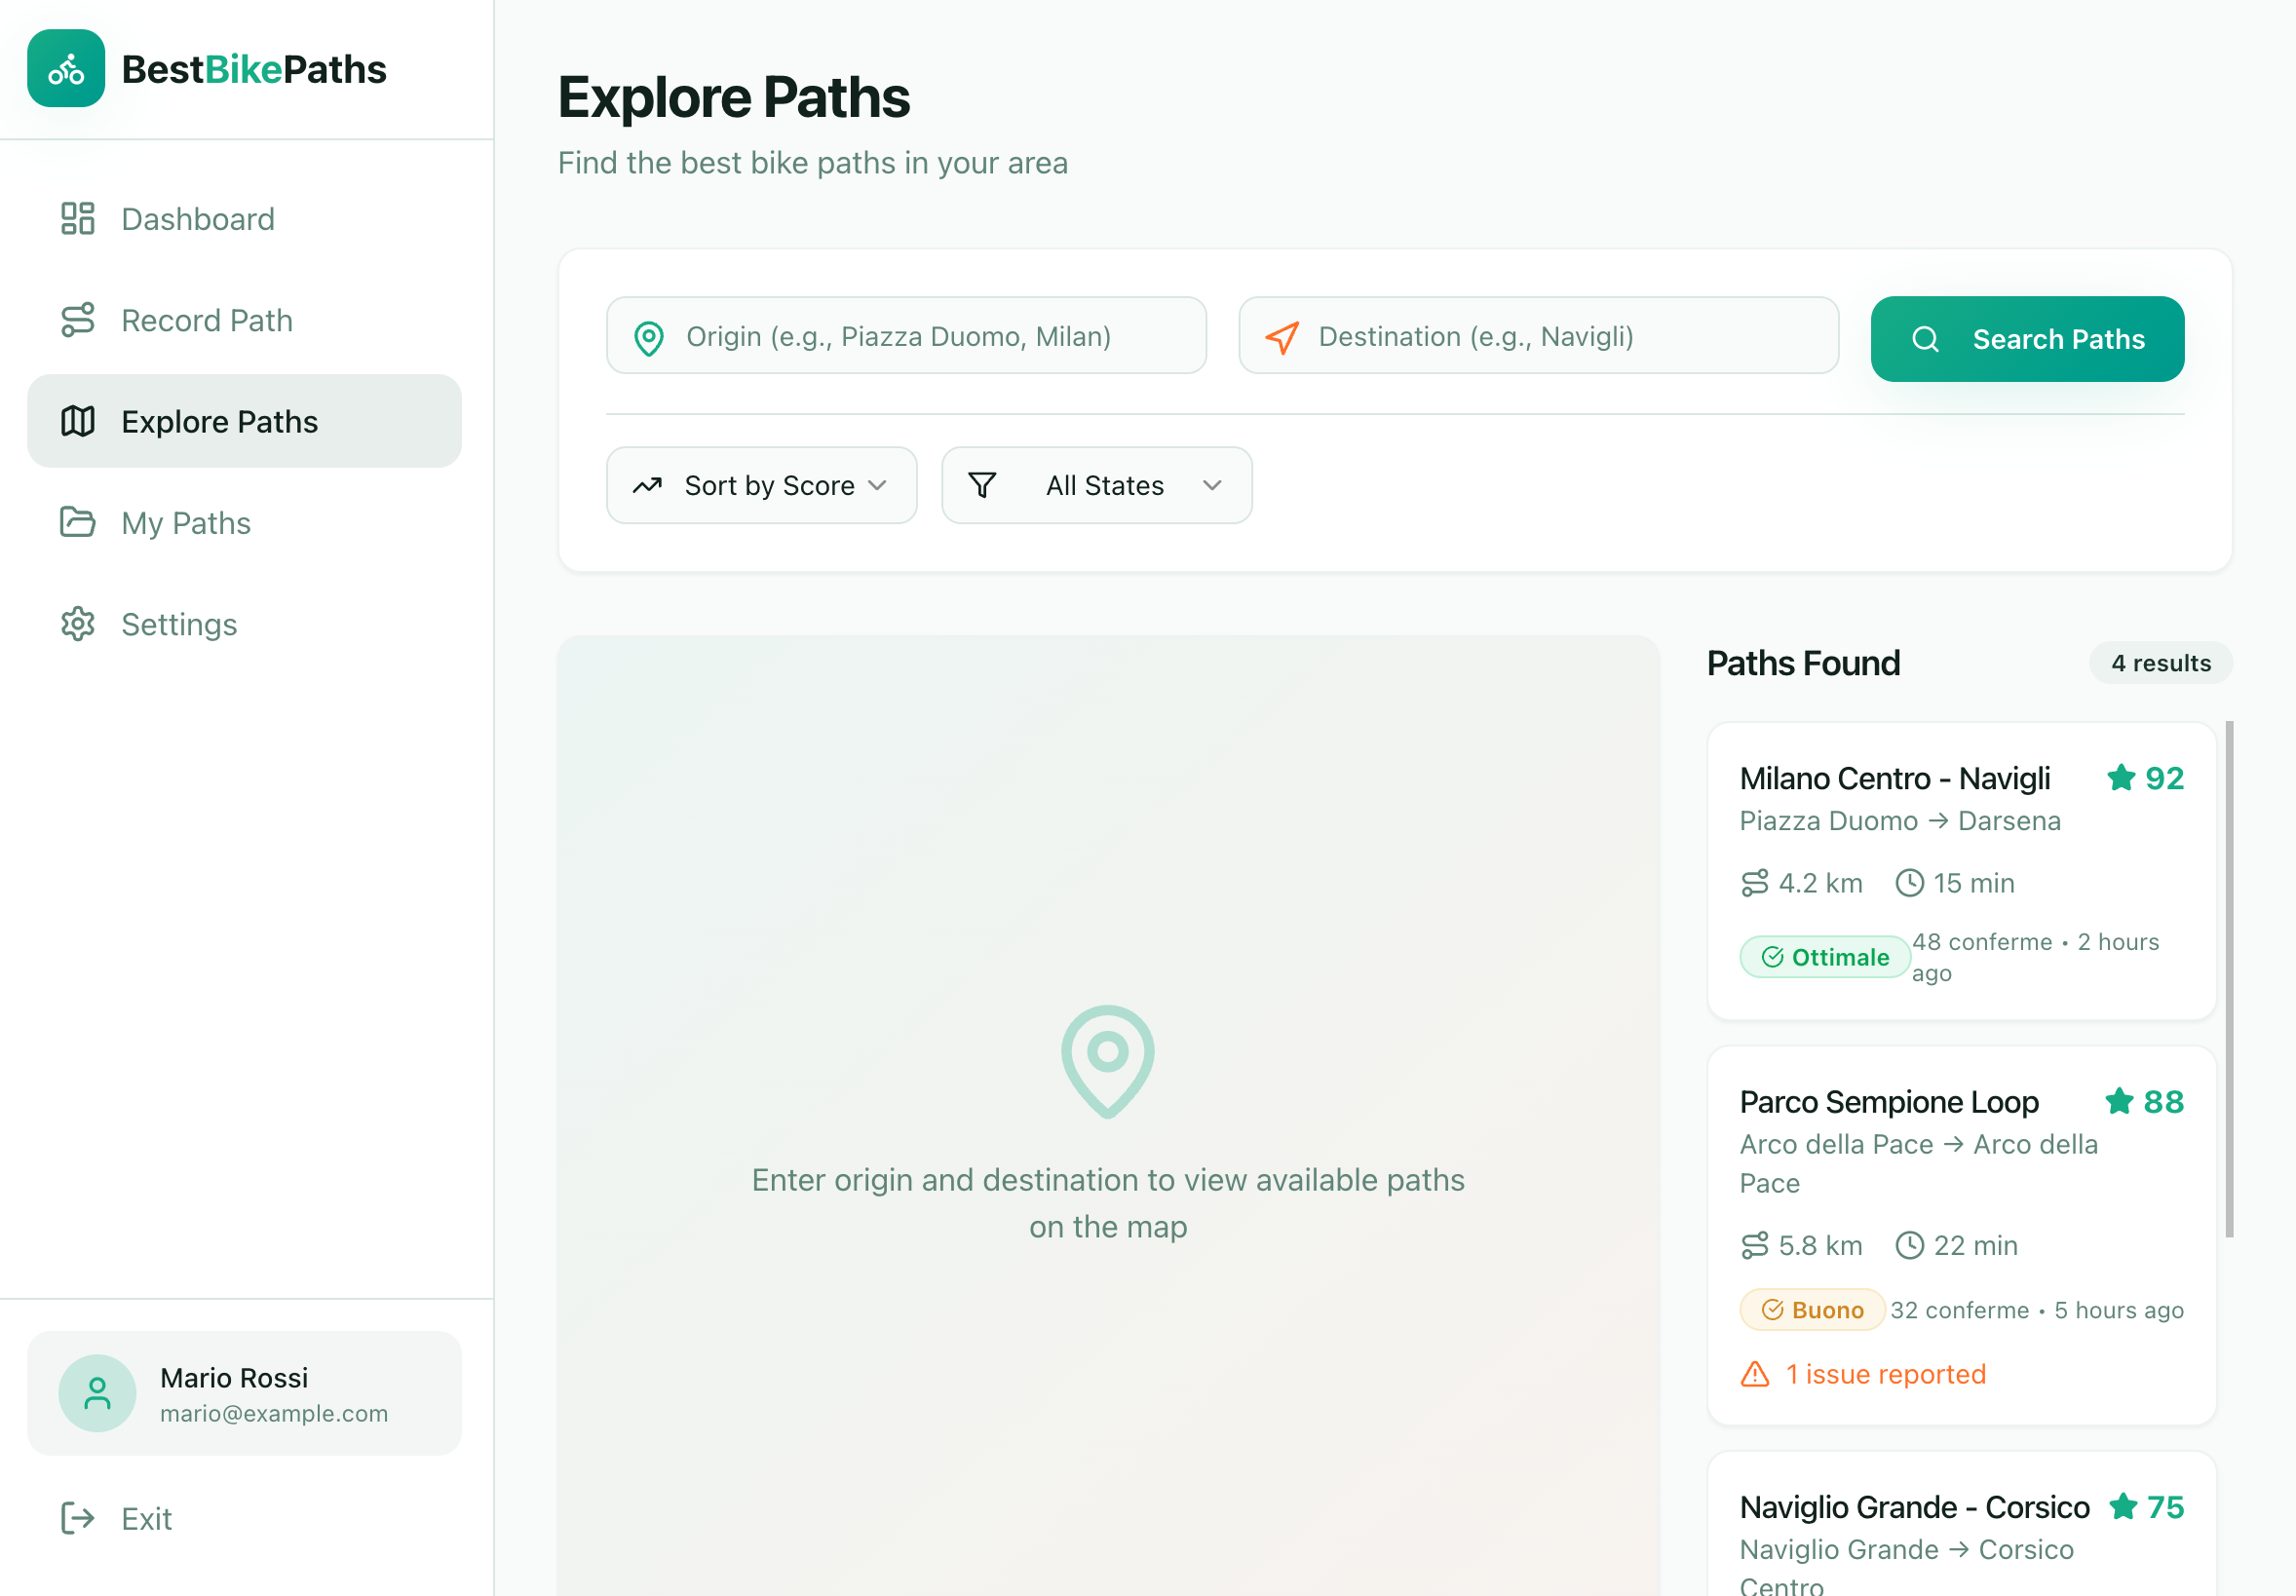
\includegraphics[width=0.8\textwidth]{Images/esplora_percorsi.png}
	\caption{Explore curated and suggested routes with filters and key stats.}
	\label{fig:esplora-percorsi}
\end{figure}
The explore view offers \textbf{curated and suggested routes} with \textbf{filters} for \textbf{difficulty}, \textbf{duration}, and \textbf{location}. Cards show a brief \textbf{description}, \textbf{tags}, and primary \textbf{stats} to help selection at a glance.

\begin{figure}[H]
	\centering
	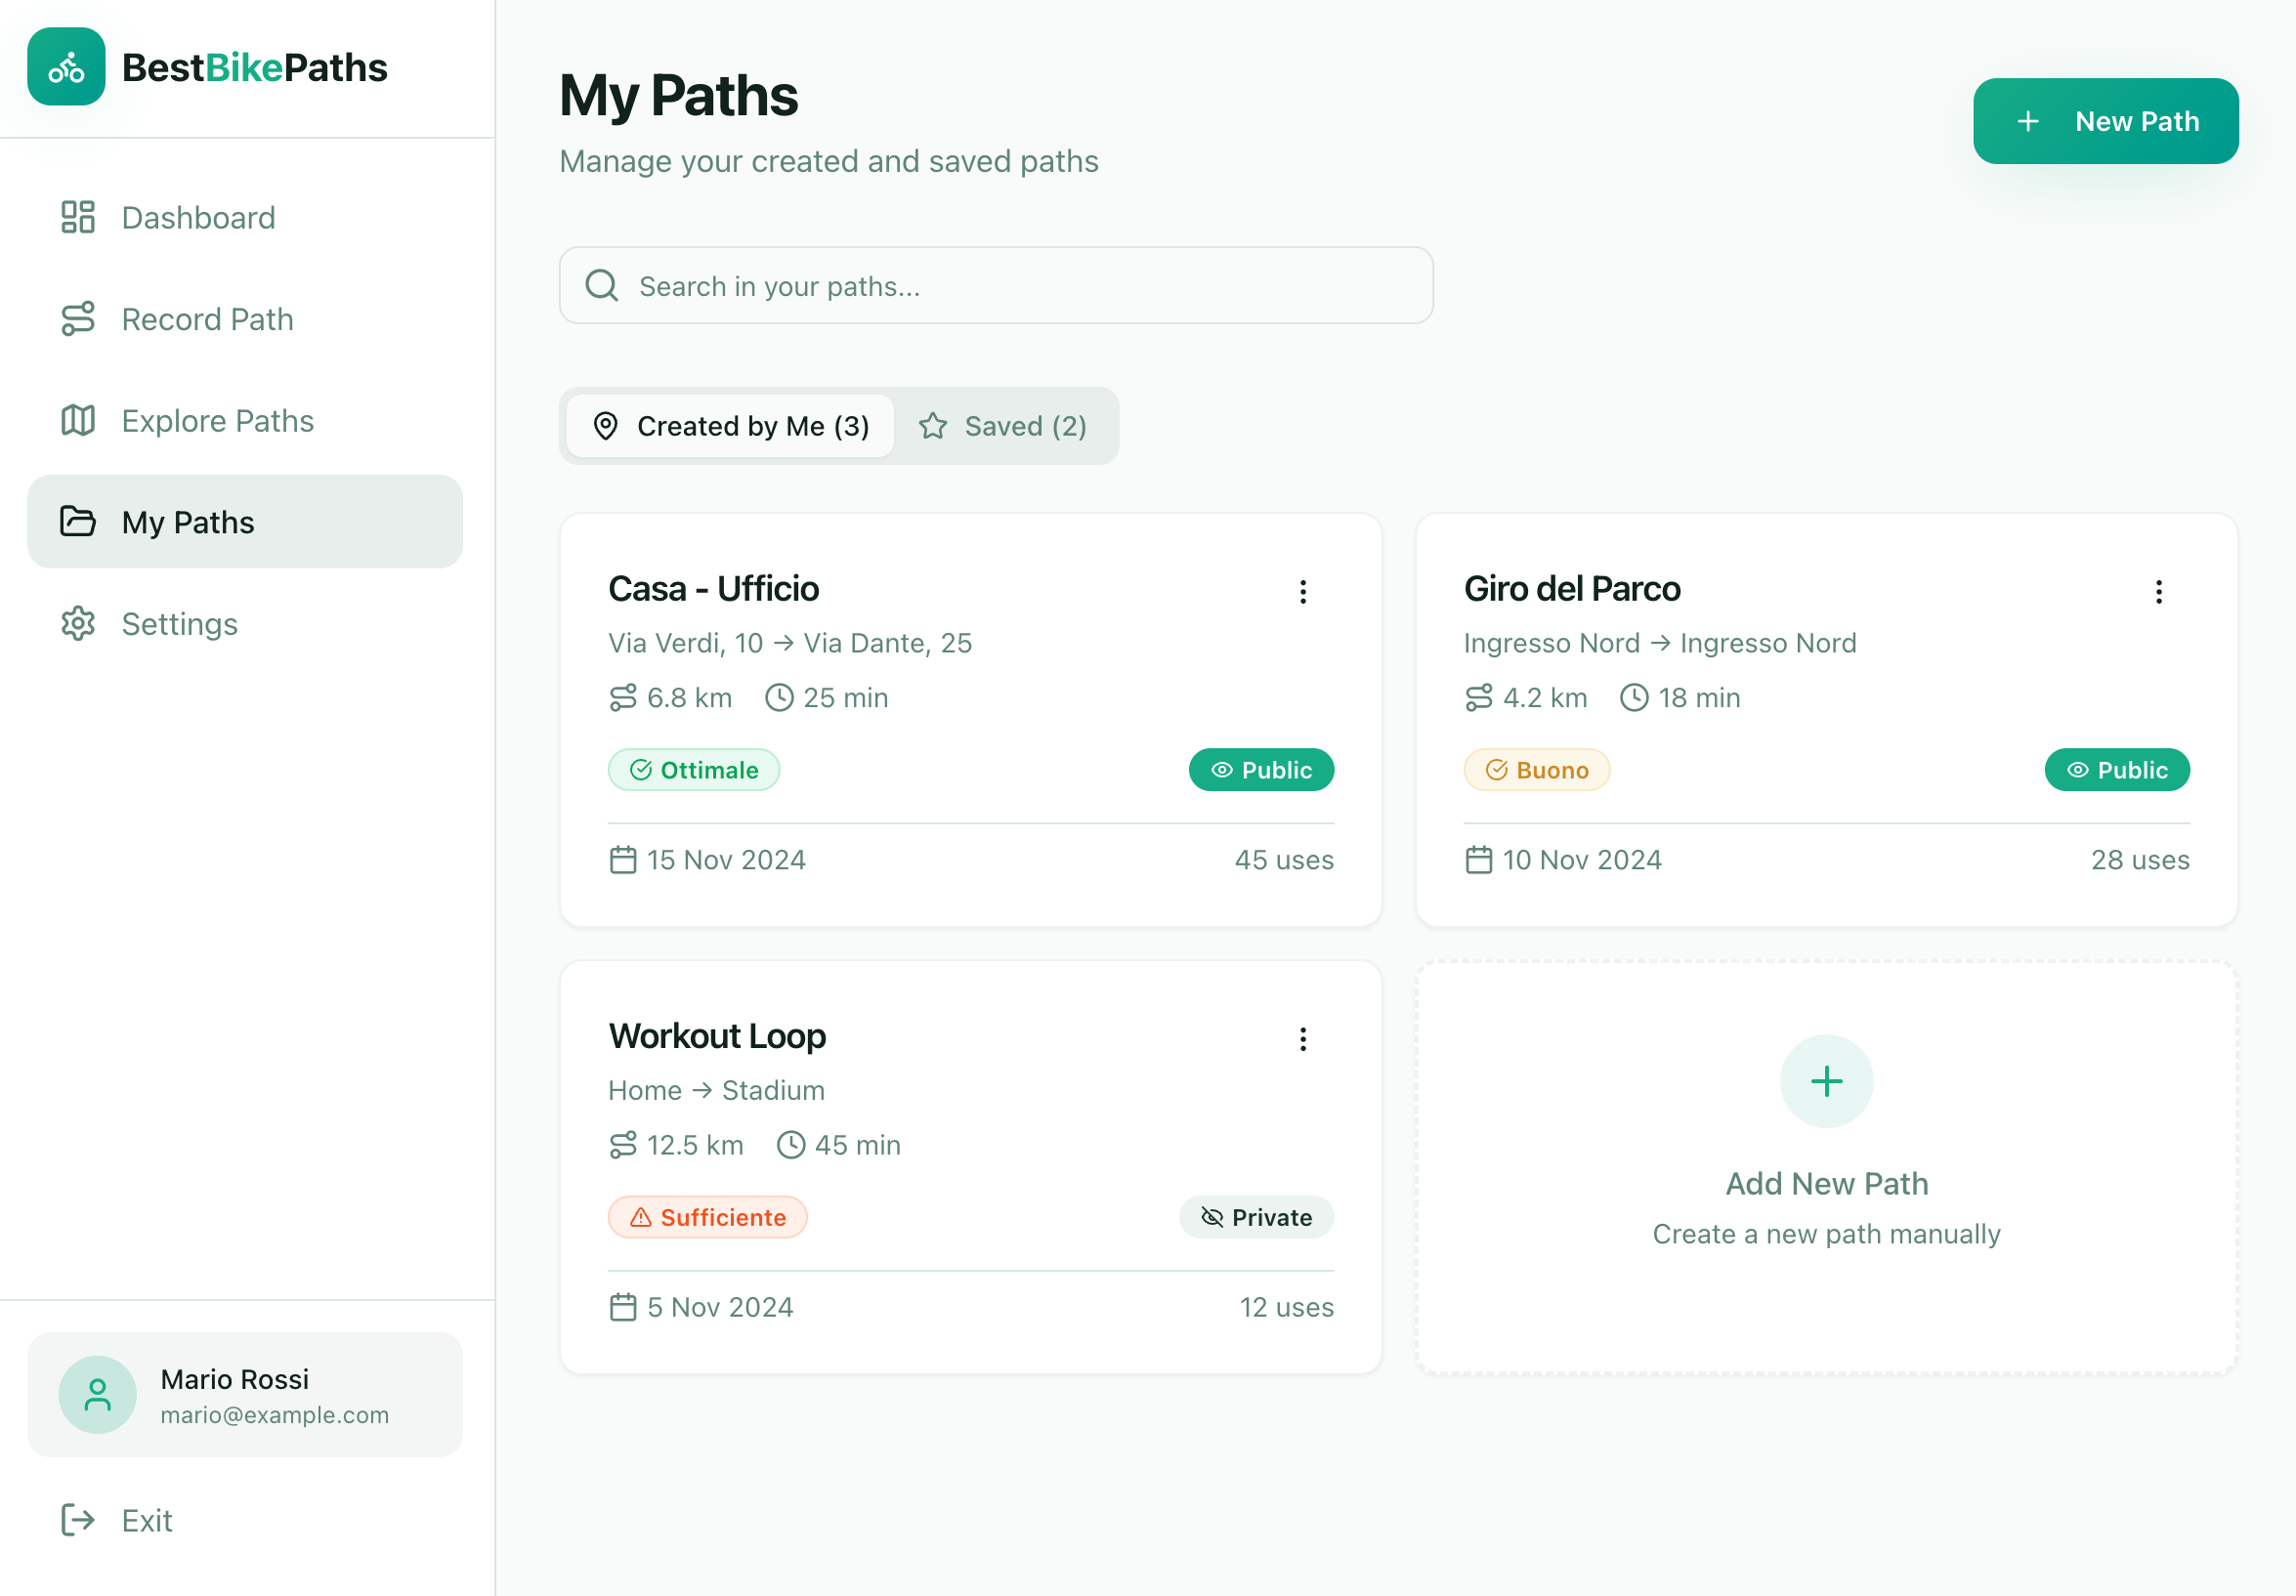
\includegraphics[width=0.8\textwidth]{Images/miei_percorsi.png}
	\caption{List of saved routes with quick access to details and navigation.}
	\label{fig:miei-percorsi}
\end{figure}

This screen lists the user \textbf{saved routes} with key \textbf{metadata} (\textbf{name}, \textbf{distance}, \textbf{duration}, \textbf{last update}) and quick entry points to view \textbf{details} or start \textbf{navigation}. Rows are designed for scannability and expose \textbf{status badges} for \textbf{drafts} or \textbf{shared items}.





\begin{figure}[H]
	\centering
	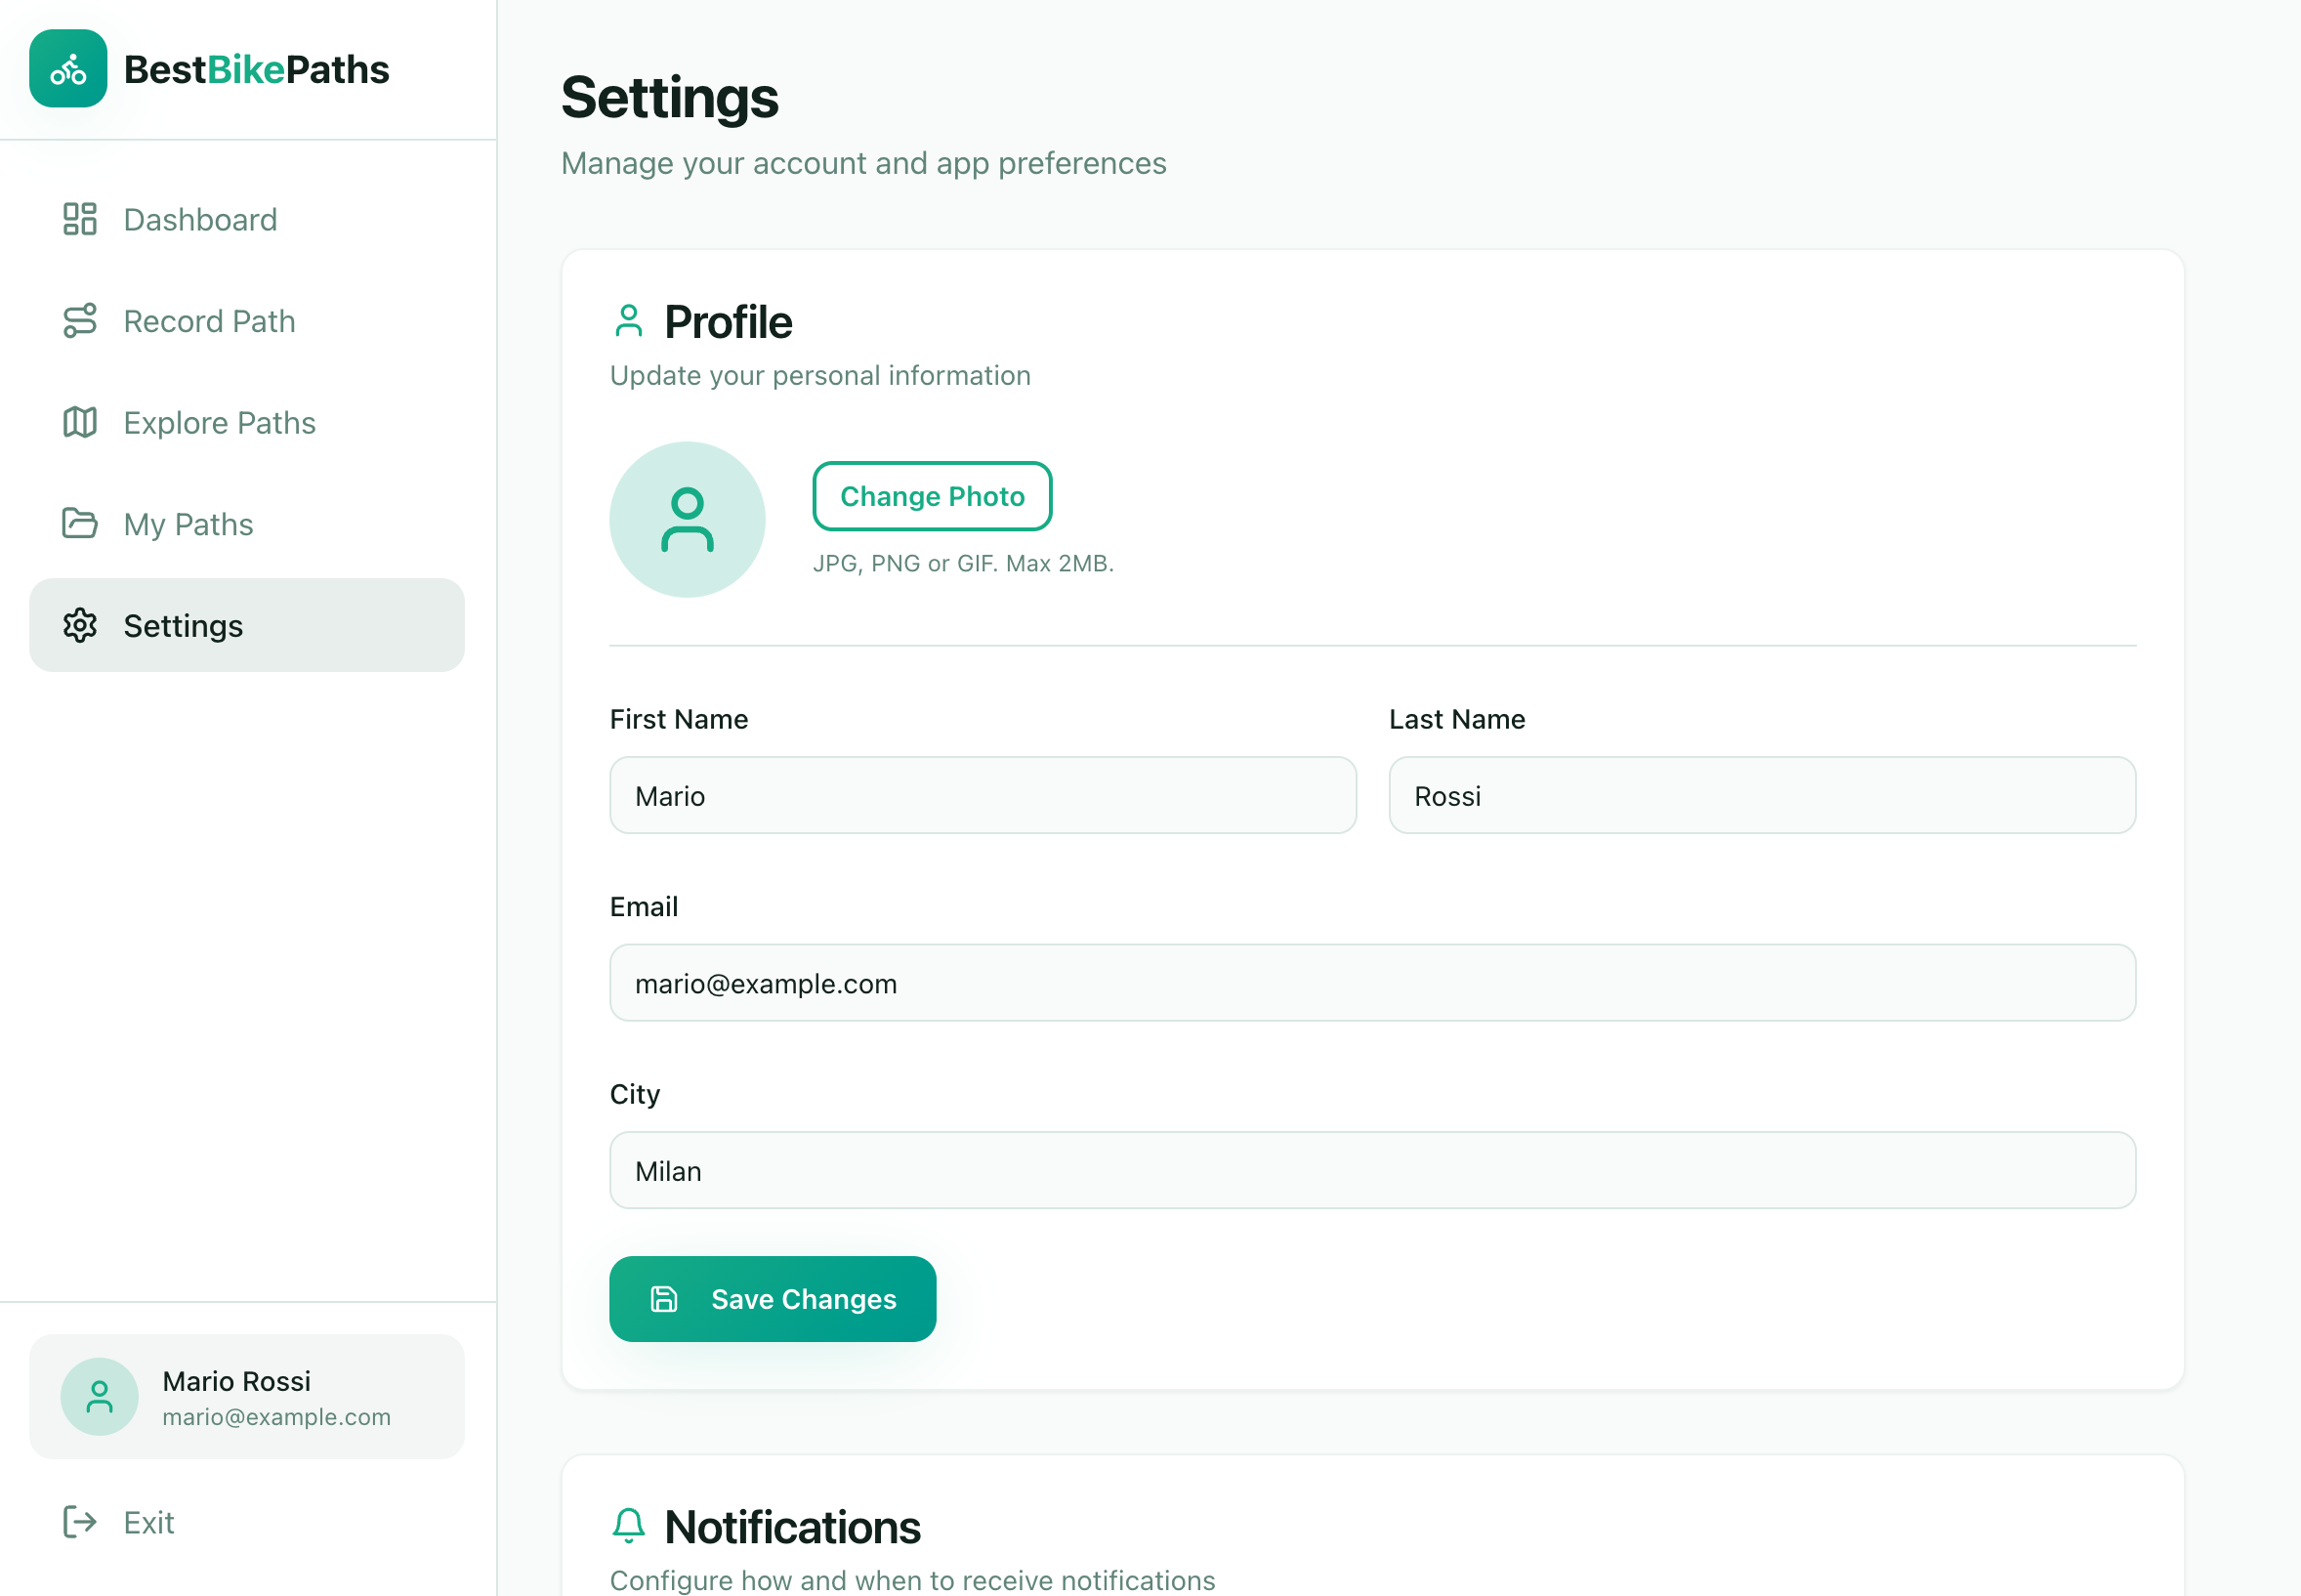
\includegraphics[width=0.8\textwidth]{Images/impostazioni.png}
	\caption{Settings grouped by account, privacy, and notifications.}
	\label{fig:impostazioni}
\end{figure}
Settings centralize \textbf{account}, \textbf{privacy}, and \textbf{notification preferences}. \textbf{Destructive actions} are visually separated.


%------------------------------------------------------------------------------------------------------------------------------------------------
\clearpage
\chapter{{Requirements Traceability}}
\label{sect:requirements_traceability}
\section{Requirements Traceability}

The following tables map the functional requirements identified in the RASD to the architectural components defined in the Design Document. This mapping ensures that every requirement is addressed by specific modules within the system.

% --- Table 1: User Account ---
\subsection{User Account Management}
\begin{table}[H]
    \centering
    \renewcommand{\arraystretch}{1.5}
    \begin{tabular}{|p{0.3\textwidth}|p{0.65\textwidth}|}
        \hline
        \textbf{Requirements} & 
        \begin{itemize}[nosep, leftmargin=*, label={}, before=\vspace{-0.6\baselineskip}, after=\strut]
            \item \textbf{R1:} The platform allows users to create an account by providing the required personal information.
            \item \textbf{R2:} The platform allows registered users to log in and access the system.
            \item \textbf{R3:} The platform allows registered users to recover the access credentials.
            \item \textbf{R4:} The platform allows guest users to access only the path search functionality.
        \end{itemize} \\
        \hline
        \textbf{Components} & 
        \begin{itemize}[nosep, leftmargin=*, before=\vspace{-0.6\baselineskip}, after=\strut]
            \item Hybrid Client App (UI)
            \item BaaS Client SDK
            \item Auth Service (Identity Provider)
            \item Spatial Database (Users Table)
        \end{itemize} \\
        \hline
    \end{tabular}
    \caption{Traceability for User Account Management}
\end{table}

% --- Table 2: Activity Recording ---
\subsection{Activity Recording}
\begin{table}[H]
    \centering
    \renewcommand{\arraystretch}{1.5}
    \begin{tabular}{|p{0.3\textwidth}|p{0.65\textwidth}|}
        \hline
        \textbf{Requirements} & 
        \begin{itemize}[nosep, leftmargin=*, label={}, before=\vspace{-0.6\baselineskip}, after=\strut]
            \item \textbf{R5:} The system shall allow registered users to start recording a new cycling activity.
            \item \textbf{R7:} The system shall collect raw data from sensors (GPS, accelerometer).
            \item \textbf{R8:} The system shall analyze speed to verify cycling activity.
            \item \textbf{R9:} The system shall analyze sensors to detect road anomalies.
            \item \textbf{R10:} The system shall calculate real-time statistics.
            \item \textbf{R11:} The system shall allow pausing and resuming.
        \end{itemize} \\
        \hline
        \textbf{Components} & 
        \begin{itemize}[nosep, leftmargin=*, before=\vspace{-0.6\baselineskip}, after=\strut]
            \item Native Bridge (Capacitor)
            \item Sensor Controller \& Filter
            \item Local Persistence Manager
            \item Map \& UI Controller
        \end{itemize} \\
        \hline
    \end{tabular}
    \caption{Traceability for Activity Recording}
\end{table}

% --- Table 3: Path Creation (Automatic) ---
\subsection{Path Creation (Automatic)}
\begin{table}[H]
    \centering
    \renewcommand{\arraystretch}{1.5}
    \begin{tabular}{|p{0.3\textwidth}|p{0.65\textwidth}|}
        \hline
        \textbf{Requirements} & 
        \begin{itemize}[nosep, leftmargin=*, label={}, before=\vspace{-0.6\baselineskip}, after=\strut]
            \item \textbf{R12:} System displays detected obstacles upon stopping activity.
            \item \textbf{R13:} System requires user validation of obstacles.
            \item \textbf{R14:} System analyzes GPS trace to match existing paths.
            \item \textbf{R15:} System associates activity with existing path if matched.
            \item \textbf{R16:} System updates status/info of existing public path.
            \item \textbf{R18:} System generates new path if no match is found.
        \end{itemize} \\
        \hline
        \textbf{Components} & 
        \begin{itemize}[nosep, leftmargin=*, before=\vspace{-0.6\baselineskip}, after=\strut]
            \item Map \& UI Controller (Validation Interface)
            \item BaaS Client SDK
            \item Spatial Database
            \item \texttt{func\_path\_merging} (Edge Function)
            \item \texttt{func\_weather\_enricher} (Edge Function)
        \end{itemize} \\
        \hline
    \end{tabular}
    \caption{Traceability for Automatic Path Creation}
\end{table}

% --- Table 4: Path Creation (Manual) ---
\subsection{Path Creation (Manual)}
\begin{table}[H]
    \centering
    \renewcommand{\arraystretch}{1.5}
    \begin{tabular}{|p{0.3\textwidth}|p{0.65\textwidth}|}
        \hline
        \textbf{Requirements} & 
        \begin{itemize}[nosep, leftmargin=*, label={}, before=\vspace{-0.6\baselineskip}, after=\strut]
            \item \textbf{R20:} User creates path manually by selecting streets on map.
            \item \textbf{R21:} User manually inputs status and obstacles.
            \item \textbf{R22:} User assigns name and stores in "My Paths".
        \end{itemize} \\
        \hline
        \textbf{Components} & 
        \begin{itemize}[nosep, leftmargin=*, before=\vspace{-0.6\baselineskip}, after=\strut]
            \item Map \& UI Controller
            \item BaaS Client SDK
            \item Spatial Database
        \end{itemize} \\
        \hline
    \end{tabular}
    \caption{Traceability for Manual Path Creation}
\end{table}

% --- Table 5: Search and Ranking ---
\subsection{Search and Ranking}
\begin{table}[H]
    \centering
    \renewcommand{\arraystretch}{1.5}
    \begin{tabular}{|p{0.3\textwidth}|p{0.65\textwidth}|}
        \hline
        \textbf{Requirements} & 
        \begin{itemize}[nosep, leftmargin=*, label={}, before=\vspace{-0.6\baselineskip}, after=\strut]
            \item \textbf{R23:} Users search paths by origin and destination.
            \item \textbf{R24:} Users filter search results.
            \item \textbf{R25:} Platform ranks paths based on condition, freshness, and effectiveness.
        \end{itemize} \\
        \hline
        \textbf{Components} & 
        \begin{itemize}[nosep, leftmargin=*, before=\vspace{-0.6\baselineskip}, after=\strut]
            \item Map \& UI Controller
            \item \texttt{func\_path\_search} (Edge Function / RPC)
            \item Spatial Database (PostGIS Indexing)
        \end{itemize} \\
        \hline
    \end{tabular}
    \caption{Traceability for Search and Ranking}
\end{table}

% --- Table 6: Path Management ---
\subsection{Path Management}
\begin{table}[H]
    \centering
    \renewcommand{\arraystretch}{1.5}
    \begin{tabular}{|p{0.3\textwidth}|p{0.65\textwidth}|}
        \hline
        \textbf{Requirements} & 
        \begin{itemize}[nosep, leftmargin=*, label={}, before=\vspace{-0.6\baselineskip}, after=\strut]
            \item \textbf{R26:} Platform detects when user follows a public path.
            \item \textbf{R27:} Users update condition info without performing activity.
            \item \textbf{R28:} Users edit info of created paths.
            \item \textbf{R29:} Users publish stored paths to community.
        \end{itemize} \\
        \hline
        \textbf{Components} & 
        \begin{itemize}[nosep, leftmargin=*, before=\vspace{-0.6\baselineskip}, after=\strut]
            \item Map \& UI Controller
            \item BaaS Client SDK
            \item Spatial Database
            \item \texttt{func\_path\_merging} (For updates/consensus)
        \end{itemize} \\
        \hline
    \end{tabular}
    \caption{Traceability for Path Management}
\end{table}
%------------------------------------------------------------------------------------------------------------------------------------------------
\clearpage
\chapter{{Implementation, Integration and Test Plan}}
\label{sect:implementation_integration_testplan}
\section{Implementation, Integration \& Testing}

\subsection{Overview}
The implementation strategy for the Best Bike Paths (BBP) system is driven by the need to combine the flexibility of web development with the performance of native hardware. The chosen architecture—Hybrid Mobile (Capacitor) supported by a Serverless Backend (Supabase + Deno)—addresses two critical requirements:

\begin{itemize}
    \item \textbf{Maximizing Data Consistency:} The pervasive use of TypeScript, from the database (via generated definitions) to the mobile client, ensures a ``Type-Safe'' ecosystem, drastically reducing integration bugs.
    \item \textbf{Optimizing Resource Usage:} By delegating spatial computational complexity to PostGIS and business logic to the Edge, the mobile client remains lightweight, preserving the user device's battery life.
\end{itemize}

\subsection{Implementation Plan}
The development process follows a ``Data-Centric Bottom-Up'' approach. Instead of starting with the user interface, implementation begins with a rigorous definition of the data model and security rules, progressively building the upper layers. This ensures that every component, once integrated, rests on a stable foundation.

\subsubsection{Phase 1: Data Integrity \& Security Layer}
The primary goal is to establish a reliable ``Single Source of Truth.'' This involves not just creating tables, but defining the data contract that will govern the entire system.

\begin{itemize}
    \item \textbf{Geospatial Persistence Engine:} The adoption of PostgreSQL with PostGIS is not merely for storage, but to serve as the primary calculation engine. Path trajectories are modeled as \texttt{GEOGRAPHY} types to ensure precise geodetic calculations (independent of map distortion), which are essential for the proximity queries required by functional requirements.
    \item \textbf{Automated Contract Generation:} To prevent misalignment between backend and frontend, a pipeline is implemented to automatically reflect the database schema into static TypeScript interfaces. This mechanism enforces that any change to the data structure (e.g., adding a ``slope'' field) is immediately propagated to the code, causing preemptive compilation errors rather than runtime failures.
    \item \textbf{Authorization at Storage Level:} Security is implemented directly on the data via Row Level Security (RLS). This ``Defense in Depth'' approach ensures that access rules (e.g., ``only the author sees private paths'') are applied universally, regardless of whether the request originates from the API, the admin dashboard, or a future client.
\end{itemize}

\subsubsection{Phase 2: Distributed Business Logic (Edge Layer)}
Application logic is developed as an intermediate layer of serverless functions (Deno), acting as intelligent glue between the client and the database.

\begin{itemize}
    \item \textbf{Compute Offloading Strategy:} Heavy operations are strategically distributed. The Database handles spatial complexity (intersections, distance calculations) via optimized RPCs. The Edge Function handles algorithmic logic (e.g., path ranking based on dynamic weights) and orchestration. This separation prevents complex calculations from blocking the main database thread or draining the smartphone's CPU.
    \item \textbf{Validation Gatekeeping:} Before any data reaches the database, it is intercepted by a validation layer (based on Zod). This component ensures the structural and semantic sanity of incoming data (e.g., verifying that a GPX track does not have impossible time jumps), protecting system integrity from malformed input or attacks.
\end{itemize}

\subsubsection{Phase 3: Hybrid Client \& Sensor Fusion}
Mobile client development focuses on hardware abstraction and offline resilience, using Capacitor as a bridge to native functionalities.

\begin{itemize}
    \item \textbf{Native Bridge Abstraction:} Capacitor is used to access critical sensors (GPS, Accelerometer), bypassing browser limitations. The goal is to ensure background execution: the system must continue recording high-frequency data even when the device is locked, a feature not reliably available in standard Web Apps.
    \item \textbf{Local-First Architecture:} Given the mobile nature of the application (usage in areas with poor coverage), the client is designed to operate autonomously. A persistent local buffer (via SQLite) is implemented to act as temporary storage.
    \item \textbf{Synchronization Logic:} An intelligent synchronization manager monitors network status. Instead of attempting immediate and fallible uploads, the system accumulates data locally and transmits it in batches to the ingestion Edge Function only when the connection is stable, implementing ``retry'' logic to ensure no activity is lost.
\end{itemize}

\subsubsection{Phase 4: Asynchronous Consistency}
The final phase handles processes that do not require real-time interaction, decoupling the user experience from heavy workloads.

\begin{itemize}
    \item \textbf{Event-Driven Updates:} To keep path statistics updated without slowing down feedback submission, an event-driven model is adopted. Inserting a new feedback asynchronously triggers (via Database Webhooks) the recalculation of the path's score. This ensures the user interface remains ``snappy'' while the system processes data in the background.
\end{itemize}

\subsection{Component Integration}
Integration in BBP is not a final phase, but a continuous process guaranteed by the architecture itself.

\begin{itemize}
    \item \textbf{Static Contract Verification:} Integration between modules (Mobile Client $\leftrightarrow$ Edge Function $\leftrightarrow$ Database) is verified statically at compile time. Sharing TypeScript types acts as a formal contract: if the database schema changes, the client will not compile until it is updated to handle the change. This eliminates entire classes of integration bugs.
    \item \textbf{Environment Parity:} To mitigate deployment risks, the local development environment faithfully replicates the production infrastructure (including containers for Edge Functions and PostGIS). This allows developers to test full flows (from simulated sensor to storage) on their own machines before even reaching the staging environment.
\end{itemize}

\subsection{Testing Strategy}
The testing strategy is designed to mitigate risks specific to an application based on geolocation and physical sensors.

\subsubsection{Logic \& Algo Testing (Unit)}
The focus is on algorithmic correctness. Since ranking and data fusion logic is isolated in pure TypeScript/Deno functions, it can be tested exhaustively with fast unit tests by mocking external dependencies. This ensures the mathematics behind score calculation is correct before involving the database.

\subsubsection{Native \& Hardware Testing (System)}
Traditional tests are insufficient to validate hardware interaction.

\begin{itemize}
    \item \textbf{Energy Profiling:} Instrumental monitoring of energy consumption is performed (via native Android/iOS profilers) to ensure background sensor sampling respects battery constraints (Requirement 3.3).
    \item \textbf{Background Lifecycle Verification:} Field tests are crucial to verify that the operating system does not ``kill'' the recording process when memory is under pressure or the screen is off for long periods.
    \item \textbf{Network Chaos:} Simulation of adverse network conditions (signal loss, switching between 4G/WiFi) to validate the robustness of the offline synchronization mechanism and prevent data loss.
\end{itemize}

%------------------------------------------------------------------------------------------------------------------------------------------------
\clearpage
\chapter{Effort Spent}
\label{sect:effort}
\begin{table}[H]
\centering
\begin{tabular}{|p{4.5cm}|l|c|c|c|}
\hline
\textbf{Chapter} & \textbf{Date} & \textbf{Alessio P.} & \textbf{Alberto S.} & \textbf{Luca S.} \\ 
\hline

% CAPITOLO 1: INTRODUCTION
\multirow{2}{=}{Introduction} 
& 29/12/2025 & 1h & 1h & - \\  
& 31/12/2025 & 1h & 1h & 1h \\
& 05/01/2026 & 1h & 1.5h & 1h \\
\cline{2-5}
& \textbf{Total} & \textbf{3h} & \textbf{3.5h} & \textbf{2h} \\ 
\hline

% CAPITOLO 2: ARCHITECTURE DESIGN
\multirow{2}{=}{Architecture Design} 
& 30/12/2025 & 1h & 3.5h & - \\ 
& 31/12/2025 & - & 2h & - \\ 
& 01/01/2026 & - & 2h & - \\ 
& 03/01/2026 & - & - & 2.5h \\
& 05/01/2026 & - & - & 2h \\
& 06/01/2026 & - & - & 2h \\
 
\cline{2-5}
& \textbf{Total} & \textbf{1h} & \textbf{7.5h} & \textbf{6.5h} \\ 
\hline

% CAPITOLO 3: USER INTERFACE DESIGN
\multirow{2}{=}{User Interface Design} 
& 05/01/2026 & 4h & - & - \\  
& 06/01/2026 & 2h & - & - \\
\cline{2-5}
& \textbf{Total} & \textbf{6h} & \textbf{0h} & \textbf{0h} \\ 
\hline

% CAPITOLO 4: REQUIREMENTS TRACEABILITY
\multirow{2}{=}{Requirements Traceability} 
& 01/01/2026 & - & 2h & - \\ 
\cline{2-5}
& \textbf{Total} & \textbf{0h} & \textbf{2h} & \textbf{0h} \\ 
\hline

% CAPITOLO 5: IMPLEMENTATION, INTEGRATION AND TEST PLAN
\multirow{2}{=}{Implementation, Integration and Test Plan} 
& 30/12/2025 & 3h & 0.5h & - \\  
\cline{2-5}
& \textbf{Total} & \textbf{3h} & \textbf{0.5h} & \textbf{0h} \\ 
\hline

\multicolumn{2}{|c|}{\textbf{TOTAL}} & \textbf{13h} & \textbf{13.5h} & \textbf{8.5h} \\
\hline

\end{tabular}
\caption{Hours of work spent by each author redacting the DD document}
\label{tab:effort}
\end{table}

\end{document}
